\documentclass[accentcolor=tud1a,colorbacktitle,inverttitle,landscape,german,presentation,t]{tudbeamer}

% usepackages
% =============================================================
\usepackage[utf8]{inputenc}
\usepackage[russian,english]{babel}

% font
\usepackage{bm}
\usepackage{pifont}
\usepackage{mxedruli}
\usepackage{soul}

% tables
\usepackage{array}
\usepackage{colortbl}
\usepackage{tabularx}
\usepackage{multirow}
\usepackage{booktabs}

\usepackage{adjustbox} 		% rotation of content

% plotting
\usepackage{tikz}
\usepackage{pgfplots}

% boxes
\usepackage[many]{tcolorbox}

% misc
\usepackage[absolute,overlay]{textpos}

% template
% =============================================================

\setbeamertemplate{section in toc}[square]

% some simple commands
% =============================================================

\newcommand{\highlight}[1]{\textcolor{tud1a}{\textbf{#1}}}

\newcommand{\gr}{\cellcolor{lightgray}}

\newcolumntype{?}{!{\vrule width 1.5pt}}

% absolute positioning of images
\newcommand{\abspos}[4]{
	\begin{textblock}{100}(#1,#2)
		\textblockcolour{white}
      		\includegraphics[scale=#4]{#3}
    	\end{textblock}
}

% divide into left and right content
\newcommand{\divideTwo}[4]{
	\begin{minipage}{#1\textwidth}
		#2
	\end{minipage}
	\hfill
	\begin{minipage}{#3\textwidth}
		#4
	\end{minipage}
}

% probing task template
\newcommand{\probingtask}[5]{
	\footnotesize
	\begin{itemize}\setlength\itemsep{1em}
		\item \textbf{Category:} \\ #1
		\item \textbf{Description:} \\ #2
		\item \textbf{Implementation:} \\ #3
		\item \textbf{Languages:} #4
		\item \textbf{Example:} \\ #5
	\end{itemize}
}

% language template
\newcommand{\lang}[5]{
	EN 	\ifnum#1=51\textcolor{green}{\ding{51}}\else\textcolor{red}{\ding{55}}\fi~~~~
	DE 	\ifnum#2=51\textcolor{green}{\ding{51}}\else\textcolor{red}{\ding{55}}\fi~~~~
	RU 	\ifnum#3=51\textcolor{green}{\ding{51}}\else\textcolor{red}{\ding{55}}\fi~~~~
	TR 	\ifnum#4=51\textcolor{green}{\ding{51}}\else\textcolor{red}{\ding{55}}\fi~~~~
	KA 	\ifnum#5=51\textcolor{green}{\ding{51}}\else\textcolor{red}{\ding{55}}\fi
}

% rotated cell content
\newcolumntype{R}[2]{%
    >{\adjustbox{angle=#1,lap=\width-(#2)}\bgroup}%
    l%
    <{\egroup}%
}
\newcommand*\rot{\multicolumn{1}{R{90}{1em}}}
\newcommand*\rotff{\multicolumn{1}{R{45}{1em}}}

% red star
\newcommand{\rs}{\textcolor{red}{\textbf{*}}}

% divider page
\newcommand{\divider}[1]{
	{\begin{frame}[plain]
		\vfill\centering
		\begin{tcolorbox}[width=4in,interior hidden,boxsep=5pt,left=0pt,right=0pt,top=2mm,
			bottom=2mm,sharp corners,colback=tud1a!40,colframe=tud1a]%%
			\centering
			\textbf{Section:} \\
			\Large \textbf{#1}
		\end{tcolorbox}
		\vfill
		\centering
		
\includegraphics[scale=0.8]{tud_logo}
		\vfill
	\end{frame}}
}

% text align
\newcommand\textalign[2][]{%
	\ifx#1l\relax
  		\makebox[0pt][l]{#2}%
	\else
  		\ifx#1r\relax
    			\makebox[0pt][r]{#2}%
  		\else  
    			\ifx#1c\relax
      				\makebox[0pt][c]{#2}%
    	\fi\fi\fi
}

% centered X column
\newcolumntype{Y}{>{\centering\arraybackslash}X}



% begin of document
% =============================================================
\begin{document}

% general information about presentation
\title[]{Interpretability of Sentence Embeddings in low-resource Languages}
\subtitle{Master thesis final presentation \\ Supervisors: Dr. Steffen Eger, Dr. Johannes Daxenberger}

\author{Daniel Wehner}
\institute[TUD UKP]{Ubiquitous Knowledge Processing, TU Darmstadt}
\logo{\color{tudtextaccent}\large UKP}
\date{October 15, 2019}

\begin{titleframe}
\end{titleframe}

% Agenda
\begin{frame}{Agenda}{}
	\tableofcontents
\end{frame}


% Section: Introduction
% ===============================================
\section{Introduction}
\divider{Introduction}

% Introduction
\begin{frame}{Introduction}{}
	\vspace*{-4mm}
	\begin{itemize}\setlength\itemsep{1em}
		\item A plethora of sentence embedding techniques has been developed
		\item \textcolor{red}{\textbf{Problem:}} \\
			\textcolor{red}{The knowledge about what is captured by sentence embeddings is limited!}
		\item \textbf{Probing tasks come to the rescue:}
		\begin{itemize}\setlength\itemsep{0.5em}
			\item \textit{`Classification problem that focuses on simple linguistic properties of sentences'} (Conneau.2018)
			\item Conneau.2018 introduced a \textbf{set of ten probing tasks}
			\item E.\,g. sentence length, containment of words, subject number, tense, etc.
			\item Conneau and colleagues mainly drew inspiration from Ettinger.2016, Shi.2016 and Adi.2017
		\end{itemize}
	\end{itemize}
\end{frame}

% Scope of this Thesis
\begin{frame}{Scope of this Thesis}{}
	\vspace*{-4mm}
	\begin{itemize}\setlength\itemsep{1em}
		\item Most research in this domain is done for English/high-resource languages
		\item \textbf{Low-resource languages are mainly neglected}
		\item Languages considered in this thesis:

		\vspace*{2mm}
		{\small
		\begin{tabbing}
			\hspace*{2.5cm}\=\hspace*{1.5cm}\=\hspace*{3.5cm}\=\kill
			\textbf{English} 		\> EN	\>									\>	high-resource	\\[2mm]
			\textbf{German}		\> DE	\> Deutsch 							\> 	high-resource	\\[2mm]
			\textbf{Russian} 	\> RU	\> \foreignlanguage{russian}{русский язык} 	\>	low-resource 	\\[2mm]
			\textbf{Turkish} 		\> TR	\> Türkçe 								\> 	low-resource 	\\[2mm]
			\textbf{Georgian}	\> KA	\> {\mxedr{kartuli ena}} 					\> 	low-resource
		\end{tabbing}}
		\item \highlight{Are patterns for English reproducible in low-resource languages?}
	\end{itemize}
\end{frame}

% Process
\begin{frame}{High-Level Process}{}
	\vspace*{-6mm}
	\begin{figure}
		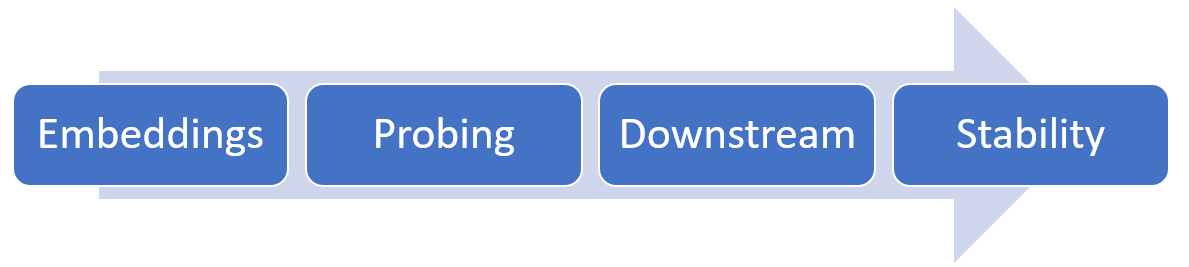
\includegraphics[scale=0.325]{images/process}
	\end{figure}

	\begin{tabbing}
		\hspace*{3cm}\=\kill
		\ding{182} \textbf{Embeddings}	\>	Train sentence encoders in multiple languages 				\\[2mm]
		\ding{183} \textbf{Probing}		\>	Data generation / Evaluation on probing tasks				\\[2mm]
		\ding{184} \textbf{Downstream}	\>	Data generation / Evaluation on downstream applications		\\[2mm]
		\ding{185} \textbf{Stability}	\>	Discrepancies with literature / different setups in literature:		\\
								\>	Investigate the rank stability of embeddings in various setups
	\end{tabbing}
\end{frame}


% Section: Sentence Embeddings
% ===============================================
\section{Sentence Embeddings}
\divider{Sentence Embeddings}

% Sentence Embedding Algorithms
\begin{frame}{Sentence Embedding Algorithms}{}
	\vspace*{-4mm}
	{\footnotesize
	\divideTwo{0.49}{
		\begin{itemize}
			\item Vanilla average (300\,d)
			\item $p$-Means (1,500\,d)
			\item Geometric embeddings (300\,d)
			\item Smooth inverse frequency (300\,d)
			\item Hierarchical pooling (300\,d)
		\end{itemize}
	}{0.49}{
		\begin{itemize}
			\item InferSent (4,096\,d)
			\item Quick-Thought (2,400\,d)
			\item sent2vec (700\,d)
			\item LASER (1,024\,d)
			\item BERT (768\,d)
			\item Random encoders (4,096/8,192\,d)
		\end{itemize}
	}}

	\begin{textblock*}{4cm}(0.75cm,5.75cm)
		\textblockcolour{tud1a!40}
		\vspace*{1mm}
		\centering
   		\textbf{Non-parametric} \strut
		\vspace*{1mm}
	\end{textblock*}

	\begin{textblock*}{4cm}(7.25cm,5.75cm)
		\textblockcolour{tud1a!40}
		\vspace*{1mm}
		\centering
   		\textbf{Parametric} \strut
		\vspace*{1mm}
	\end{textblock*}

	\vspace*{1.5cm}
	\begin{itemize}\setlength\itemsep{1em}
		\item Non-parametric: Aggregation of word embeddings \textbf{without training}
		\item Parametric models are \textbf{trained from scratch} on top of word embeddings
	\end{itemize}
\end{frame}


% Section: Probing and Downstream Tasks
% ===============================================
\section{Probing and Downstream Tasks}
\divider{Probing and Downstream Tasks}

% Probing Tasks
\begin{frame}{Probing Task Examples}{}
	\vspace*{-4mm}
	\begin{itemize}\setlength\itemsep{1em}
		\item \highlight{Sentence Length (\caps{SentLen}):} \\ \vspace*{2mm}
		\begin{tabbing}
			\hspace*{4cm}\=\kill
				E.\,g.: \textbf{Label:} \textit{short} \> \textbf{Sentence:} \textit{It felt good to smile .} \\
			{\footnotesize (A binning approach is used for the labels.
			Think of classes like \textit{`short'}, \textit{`medium'}, \textit{`long'})}
		\end{tabbing}\vspace*{2mm}
		\item \highlight{Word Content (\caps{WC}):} \\ \vspace*{2mm}
		\begin{tabbing}
			\hspace*{4cm}\=\kill
			E.\,g.: \textbf{Label:} \textit{everybody} \> \textbf{Sentence:} \textit{Everybody should step back .}
		\end{tabbing}\vspace*{2mm}
		\item \highlight{Subject-Verb Agreement (\caps{SVAgree}):} \\ \vspace*{2mm}
		\begin{tabbing}
			\hspace*{4cm}\=\kill
			E.\,g.: \textbf{Label:} \textit{disagree} \> \textbf{Sentence:} \textit{They work\textcolor{red}{s} together .}
		\end{tabbing}
	\end{itemize}
\end{frame}

% Probing Task Setup
\begin{frame}{Probing Task Setup}{}
	\vspace*{-4mm}
	\begin{itemize}\setlength\itemsep{1em}
		\item Implementation of 9 probing tasks for EN, DE, RU, TR as well as 7 for KA \\
			{\footnotesize (\caps{SentLen}, \caps{WC}, \caps{BiShift}, \caps{SVAgree}, \caps{SVDist}\rs,
			\caps{Voice}, \caps{WO}, \caps{EOS} and \caps{SubjNum}\rs)}
		\item \highlight{New:} \caps{SVAgree} and \caps{SVDist} \textit{(inspired by Linzen.2016)}
		\item Many tasks require corpora with \textbf{morpho-syntactic} annotations
		\item Universal Dependencies offers tree banks for many languages / GNC
		\item \textbf{Evaluation: MLP with 5-fold x-val}
		\begin{itemize}
			\item One hidden layer with 50 hidden units
			\item Dropout: 0.00
			\item Activation: Sigmoid
			\item Optimizer: Adam
		\end{itemize}
	\end{itemize}

	\vfill
	{\footnotesize \rs\ not implemented for KA}
\end{frame}

% Probing Task Results English
\begin{frame}{Probing Task Results for English}{}
	\vspace*{-6mm}
	\begin{minipage}{0.115\textwidth}
\begin{tikzpicture}[scale=0.75,every node/.style={scale=0.8}]

  	\begin{axis}[
		title=SentLen\strut,
 	   	xbar stacked,
		bar width=4pt,
		enlarge y limits=0.2,
    		symbolic y coords={rand. BiLSTM,InferSent,Laser,Bert,Quick-Th.,sent2vec,p-Means,Average},
		xmin=0,xmax=1,
  		xmajorgrids,
		tickwidth=0pt,
		xtick distance=0.40,
  		ytick=data,
		scale only axis=true,
  		width=1.3cm,height=2.75cm,
		tick label style={font=\footnotesize}
  	]

		% Average
  		\addplot[blue,fill,draw=black] coordinates
  			{(0.240,Average) (0.00,p-Means) (0.00,sent2vec) (0.00,Quick-Th.) (0.00,Bert) (0.00,Laser) (0.00,InferSent) (0.00,rand. BiLSTM)};
		% p-Means
		\addplot[blue!50,fill,draw=black] coordinates
			{(0.00,Average) (0.553,p-Means) (0.00,sent2vec) (0.00,Quick-Th.) (0.00,Bert) (0.00,Laser) (0.00,InferSent) (0.00,rand. BiLSTM)};

		% sent2vec
		\addplot[red,fill,draw=black] coordinates 
			{(0.00,Average) (0.00,p-Means) (0.254,sent2vec) (0.00,Quick-Th.) (0.00,Bert) (0.00,Laser) (0.00,InferSent) (0.00,rand. BiLSTM)};
		% Quick-Th.
		\addplot[red!60,fill,draw=black] coordinates
			{(0.00,Average) (0.00,p-Means) (0.00,sent2vec) (0.649,Quick-Th.) (0.00,Bert) (0.00,Laser) (0.00,InferSent) (0.00,rand. BiLSTM)};
		% Bert
		\addplot[red!40,fill,draw=black] coordinates
			{(0.00,Average) (0.00,p-Means) (0.00,sent2vec) (0.00,Quick-Th.) (0.551,Bert) (0.00,Laser) (0.00,InferSent) (0.00,rand. BiLSTM)};
		% Laser
		\addplot[red!20,fill,draw=black] coordinates
			{(0.00,Average) (0.00,p-Means) (0.00,sent2vec) (0.00,Quick-Th.) (0.00,Bert) (0.697,Laser) (0.00,InferSent) (0.00,rand. BiLSTM)};
		% InferSentent
		\addplot[red!10,fill,draw=black] coordinates
			{(0.00,Average) (0.00,p-Means) (0.00,sent2vec) (0.00,Quick-Th.) (0.00,Bert) (0.00,Laser) (0.600,InferSent) (0.00,rand. BiLSTM)};

		% rand lstm
		\addplot[gray,fill,draw=black] coordinates 
			{(0.00,Average) (0.00,p-Means) (0.00,sent2vec) (0.00,Quick-Th.) (0.00,Bert) (0.00,Laser) (0.00,InferSent) (0.549,rand. BiLSTM)};

  	\end{axis}

\end{tikzpicture}
\end{minipage}
\hspace*{17mm}
\begin{minipage}{0.09\textwidth}
\begin{tikzpicture}[scale=0.75,every node/.style={scale=0.8}]

  	\begin{axis}[
		title=WC\strut,
   	 	xbar stacked,
		bar width=4pt,
		enlarge y limits=0.2,
	    	symbolic y coords={rand. BiLSTM,InferSent,Laser,Bert,Quick-Th.,sent2vec,p-Means,Average},
		xmin=0,xmax=1,
  		xmajorgrids,
		tickwidth=0pt,
		xtick distance=0.40,
  		ytick=data,
		yticklabels={,,},
		scale only axis=true,
  		width=1.3cm,height=2.75cm,
		tick label style={font=\footnotesize}
  	]

		% Average
  		\addplot[blue,fill,draw=black] coordinates
  			{(0.581,Average) (0.00,p-Means) (0.00,sent2vec) (0.00,Quick-Th.) (0.00,Bert) (0.00,Laser) (0.00,InferSent) (0.00,rand. BiLSTM)};
		% p-Means
		\addplot[blue!50,fill,draw=black] coordinates
			{(0.00,Average) (0.657,p-Means) (0.00,sent2vec) (0.00,Quick-Th.) (0.00,Bert) (0.00,Laser) (0.00,InferSent) (0.00,rand. BiLSTM)};

		% sent2vec
		\addplot[red,fill,draw=black] coordinates 
			{(0.00,Average) (0.00,p-Means) (0.786,sent2vec) (0.00,Quick-Th.) (0.00,Bert) (0.00,Laser) (0.00,InferSent) (0.00,rand. BiLSTM)};
		% Quick-Th.
		\addplot[red!60,fill,draw=black] coordinates
			{(0.00,Average) (0.00,p-Means) (0.00,sent2vec) (0.848,Quick-Th.) (0.00,Bert) (0.00,Laser) (0.00,InferSent) (0.00,rand. BiLSTM)};
		% Bert
		\addplot[red!40,fill,draw=black] coordinates
			{(0.00,Average) (0.00,p-Means) (0.00,sent2vec) (0.00,Quick-Th.) (0.531,Bert) (0.00,Laser) (0.00,InferSent) (0.00,rand. BiLSTM)};
		% Laser
		\addplot[red!20,fill,draw=black] coordinates
			{(0.00,Average) (0.00,p-Means) (0.00,sent2vec) (0.00,Quick-Th.) (0.00,Bert) (0.832,Laser) (0.00,InferSent) (0.00,rand. BiLSTM)};
		% InferSentent
		\addplot[red!10,fill,draw=black] coordinates
			{(0.00,Average) (0.00,p-Means) (0.00,sent2vec) (0.00,Quick-Th.) (0.00,Bert) (0.00,Laser) (0.919,InferSent) (0.00,rand. BiLSTM)};

		% rand lstm
		\addplot[gray,fill,draw=black] coordinates 
			{(0.00,Average) (0.00,p-Means) (0.00,sent2vec) (0.00,Quick-Th.) (0.00,Bert) (0.00,Laser) (0.00,InferSent) (0.462,rand. BiLSTM)};

  	\end{axis}

\end{tikzpicture}
\end{minipage}
\hspace*{10mm}
\begin{minipage}{0.09\textwidth}
\begin{tikzpicture}[scale=0.75,every node/.style={scale=0.8}]

  	\begin{axis}[
		title=BiShift\strut,
 	   	xbar stacked,
		bar width=4pt,
		enlarge y limits=0.2,
    		symbolic y coords={rand. BiLSTM,InferSent,Laser,Bert,Quick-Th.,sent2vec,p-Means,Average},
		xmin=0,xmax=1,
  		xmajorgrids,
		tickwidth=0pt,
		xtick distance=0.40,
  		ytick=data,
		yticklabels={,,},
		scale only axis=true,
  		width=1.3cm,height=2.75cm,
		tick label style={font=\footnotesize}
  	]

		% Average
  		\addplot[blue,fill,draw=black] coordinates
  			{(0.485,Average) (0.00,p-Means) (0.00,sent2vec) (0.00,Quick-Th.) (0.00,Bert) (0.00,Laser) (0.00,InferSent) (0.00,rand. BiLSTM)};
		% p-Means
		\addplot[blue!50,fill,draw=black] coordinates
			{(0.00,Average) (0.491,p-Means) (0.00,sent2vec) (0.00,Quick-Th.) (0.00,Bert) (0.00,Laser) (0.00,InferSent) (0.00,rand. BiLSTM)};

		% sent2vec
		\addplot[red,fill,draw=black] coordinates 
			{(0.00,Average) (0.00,p-Means) (0.534,sent2vec) (0.00,Quick-Th.) (0.00,Bert) (0.00,Laser) (0.00,InferSent) (0.00,rand. BiLSTM)};
		% Quick-Th.
		\addplot[red!60,fill,draw=black] coordinates
			{(0.00,Average) (0.00,p-Means) (0.00,sent2vec) (0.544,Quick-Th.) (0.00,Bert) (0.00,Laser) (0.00,InferSent) (0.00,rand. BiLSTM)};
		% Bert
		\addplot[red!40,fill,draw=black] coordinates
			{(0.00,Average) (0.00,p-Means) (0.00,sent2vec) (0.00,Quick-Th.) (0.641,Bert) (0.00,Laser) (0.00,InferSent) (0.00,rand. BiLSTM)};
		% Laser
		\addplot[red!20,fill,draw=black] coordinates
			{(0.00,Average) (0.00,p-Means) (0.00,sent2vec) (0.00,Quick-Th.) (0.00,Bert) (0.600,Laser) (0.00,InferSent) (0.00,rand. BiLSTM)};
		% InferSentent
		\addplot[red!10,fill,draw=black] coordinates
			{(0.00,Average) (0.00,p-Means) (0.00,sent2vec) (0.00,Quick-Th.) (0.00,Bert) (0.00,Laser) (0.536,InferSent) (0.00,rand. BiLSTM)};

		% rand lstm
		\addplot[gray,fill,draw=black] coordinates 
			{(0.00,Average) (0.00,p-Means) (0.00,sent2vec) (0.00,Quick-Th.) (0.00,Bert) (0.00,Laser) (0.00,InferSent) (0.510,rand. BiLSTM)};

  	\end{axis}

\end{tikzpicture}
\end{minipage}
\hspace*{10mm}
\begin{minipage}{0.09\textwidth}
\begin{tikzpicture}[scale=0.75,every node/.style={scale=0.8}]

  	\begin{axis}[
		title=SVAgree\strut,
 	   	xbar stacked,
		bar width=4pt,
		enlarge y limits=0.2,
    		symbolic y coords={rand. BiLSTM,InferSent,Laser,Bert,Quick-Th.,sent2vec,p-Means,Average},
		xmin=0,xmax=1,
  		xmajorgrids,
		tickwidth=0pt,
		xtick distance=0.40,
  		ytick=data,
		yticklabels={,,},
		scale only axis=true,
  		width=1.3cm,height=2.75cm,
		tick label style={font=\footnotesize}
  	]

		% Average
  		\addplot[blue,fill,draw=black] coordinates
  			{(0.775,Average) (0.00,p-Means) (0.00,sent2vec) (0.00,Quick-Th.) (0.00,Bert) (0.00,Laser) (0.00,InferSent) (0.00,rand. BiLSTM)};
		% p-Means
		\addplot[blue!50,fill,draw=black] coordinates
			{(0.00,Average) (0.804,p-Means) (0.00,sent2vec) (0.00,Quick-Th.) (0.00,Bert) (0.00,Laser) (0.00,InferSent) (0.00,rand. BiLSTM)};

		% sent2vec
		\addplot[red,fill,draw=black] coordinates 
			{(0.00,Average) (0.00,p-Means) (0.910,sent2vec) (0.00,Quick-Th.) (0.00,Bert) (0.00,Laser) (0.00,InferSent) (0.00,rand. BiLSTM)};
		% Quick-Th.
		\addplot[red!60,fill,draw=black] coordinates
			{(0.00,Average) (0.00,p-Means) (0.00,sent2vec) (0.887,Quick-Th.) (0.00,Bert) (0.00,Laser) (0.00,InferSent) (0.00,rand. BiLSTM)};
		% Bert
		\addplot[red!40,fill,draw=black] coordinates
			{(0.00,Average) (0.00,p-Means) (0.00,sent2vec) (0.00,Quick-Th.) (0.718,Bert) (0.00,Laser) (0.00,InferSent) (0.00,rand. BiLSTM)};
		% Laser
		\addplot[red!20,fill,draw=black] coordinates
			{(0.00,Average) (0.00,p-Means) (0.00,sent2vec) (0.00,Quick-Th.) (0.00,Bert) (0.572,Laser) (0.00,InferSent) (0.00,rand. BiLSTM)};
		% InferSentent
		\addplot[red!10,fill,draw=black] coordinates
			{(0.00,Average) (0.00,p-Means) (0.00,sent2vec) (0.00,Quick-Th.) (0.00,Bert) (0.00,Laser) (0.912,InferSent) (0.00,rand. BiLSTM)};

		% rand lstm
		\addplot[gray,fill,draw=black] coordinates 
			{(0.00,Average) (0.00,p-Means) (0.00,sent2vec) (0.00,Quick-Th.) (0.00,Bert) (0.00,Laser) (0.00,InferSent) (0.819,rand. BiLSTM)};

  	\end{axis}

\end{tikzpicture}
\end{minipage}

\vspace*{3mm}
\begin{minipage}{0.09\textwidth}
\begin{tikzpicture}[scale=0.75,every node/.style={scale=0.8}]

  	\begin{axis}[
		title=SVDist\strut,
 	   	xbar stacked,
		bar width=4pt,
		enlarge y limits=0.2,
    		symbolic y coords={rand. BiLSTM,InferSent,Laser,Bert,Quick-Th.,sent2vec,p-Means,Average},
		xmin=0,xmax=1,
  		xmajorgrids,
		tickwidth=0pt,
		xtick distance=0.40,
  		ytick=data,
		scale only axis=true,
  		width=1.3cm,height=2.75cm,
		tick label style={font=\footnotesize}
  	]

		% Average
  		\addplot[blue,fill,draw=black] coordinates
  			{(0.265,Average) (0.00,p-Means) (0.00,sent2vec) (0.00,Quick-Th.) (0.00,Bert) (0.00,Laser) (0.00,InferSent) (0.00,rand. BiLSTM)};
		% p-Means
		\addplot[blue!50,fill,draw=black] coordinates
			{(0.00,Average) (0.309,p-Means) (0.00,sent2vec) (0.00,Quick-Th.) (0.00,Bert) (0.00,Laser) (0.00,InferSent) (0.00,rand. BiLSTM)};

		% sent2vec
		\addplot[red,fill,draw=black] coordinates 
			{(0.00,Average) (0.00,p-Means) (0.301,sent2vec) (0.00,Quick-Th.) (0.00,Bert) (0.00,Laser) (0.00,InferSent) (0.00,rand. BiLSTM)};
		% Quick-Th.
		\addplot[red!60,fill,draw=black] coordinates
			{(0.00,Average) (0.00,p-Means) (0.00,sent2vec) (0.410,Quick-Th.) (0.00,Bert) (0.00,Laser) (0.00,InferSent) (0.00,rand. BiLSTM)};
		% Bert
		\addplot[red!40,fill,draw=black] coordinates
			{(0.00,Average) (0.00,p-Means) (0.00,sent2vec) (0.00,Quick-Th.) (0.406,Bert) (0.00,Laser) (0.00,InferSent) (0.00,rand. BiLSTM)};
		% Laser
		\addplot[red!20,fill,draw=black] coordinates
			{(0.00,Average) (0.00,p-Means) (0.00,sent2vec) (0.00,Quick-Th.) (0.00,Bert) (0.521,Laser) (0.00,InferSent) (0.00,rand. BiLSTM)};
		% InferSentent
		\addplot[red!10,fill,draw=black] coordinates
			{(0.00,Average) (0.00,p-Means) (0.00,sent2vec) (0.00,Quick-Th.) (0.00,Bert) (0.00,Laser) (0.414,InferSent) (0.00,rand. BiLSTM)};

		% rand lstm
		\addplot[gray,fill,draw=black] coordinates 
			{(0.00,Average) (0.00,p-Means) (0.00,sent2vec) (0.00,Quick-Th.) (0.00,Bert) (0.00,Laser) (0.00,InferSent) (0.323,rand. BiLSTM)};

  	\end{axis}

\end{tikzpicture}
\end{minipage}
\hspace*{19.75mm}
\begin{minipage}{0.09\textwidth}
\begin{tikzpicture}[scale=0.75,every node/.style={scale=0.8}]

  	\begin{axis}[
		title=Voice\strut,
    		xbar stacked,
		bar width=4pt,
		enlarge y limits=0.2,
    		symbolic y coords={rand. BiLSTM,InferSent,Laser,Bert,Quick-Th.,sent2vec,p-Means,Average},
		xmin=0,xmax=1,
  		xmajorgrids,
		tickwidth=0pt,
		xtick distance=0.40,
  		ytick=data,
		yticklabels={,,},
		scale only axis=true,
  		width=1.3cm,height=2.75cm,
		tick label style={font=\footnotesize}
  	]

		% Average
  		\addplot[blue,fill,draw=black] coordinates
  			{(0.798,Average) (0.00,p-Means) (0.00,sent2vec) (0.00,Quick-Th.) (0.00,Bert) (0.00,Laser) (0.00,InferSent) (0.00,rand. BiLSTM)};
		% p-Means
		\addplot[blue!50,fill,draw=black] coordinates
			{(0.00,Average) (0.807,p-Means) (0.00,sent2vec) (0.00,Quick-Th.) (0.00,Bert) (0.00,Laser) (0.00,InferSent) (0.00,rand. BiLSTM)};

		% sent2vec
		\addplot[red,fill,draw=black] coordinates 
			{(0.00,Average) (0.00,p-Means) (0.779,sent2vec) (0.00,Quick-Th.) (0.00,Bert) (0.00,Laser) (0.00,InferSent) (0.00,rand. BiLSTM)};
		% Quick-Th.
		\addplot[red!60,fill,draw=black] coordinates
			{(0.00,Average) (0.00,p-Means) (0.00,sent2vec) (0.811,Quick-Th.) (0.00,Bert) (0.00,Laser) (0.00,InferSent) (0.00,rand. BiLSTM)};
		% Bert
		\addplot[red!40,fill,draw=black] coordinates
			{(0.00,Average) (0.00,p-Means) (0.00,sent2vec) (0.00,Quick-Th.) (0.760,Bert) (0.00,Laser) (0.00,InferSent) (0.00,rand. BiLSTM)};
		% Laser
		\addplot[red!20,fill,draw=black] coordinates
			{(0.00,Average) (0.00,p-Means) (0.00,sent2vec) (0.00,Quick-Th.) (0.00,Bert) (0.904,Laser) (0.00,InferSent) (0.00,rand. BiLSTM)};
		% InferSentent
		\addplot[red!10,fill,draw=black] coordinates
			{(0.00,Average) (0.00,p-Means) (0.00,sent2vec) (0.00,Quick-Th.) (0.00,Bert) (0.00,Laser) (0.868,InferSent) (0.00,rand. BiLSTM)};

		% rand lstm
		\addplot[gray,fill,draw=black] coordinates 
			{(0.00,Average) (0.00,p-Means) (0.00,sent2vec) (0.00,Quick-Th.) (0.00,Bert) (0.00,Laser) (0.00,InferSent) (0.833,rand. BiLSTM)};

  	\end{axis}

\end{tikzpicture}
\end{minipage}
\hspace*{10mm}
\begin{minipage}{0.09\textwidth}
\begin{tikzpicture}[scale=0.75,every node/.style={scale=0.8}]

  	\begin{axis}[
		title=WO\strut,
   	 	xbar stacked,
		bar width=4pt,
		enlarge y limits=0.2,
    		symbolic y coords={rand. BiLSTM,InferSent,Laser,Bert,Quick-Th.,sent2vec,p-Means,Average},
		xmin=0,xmax=1,
  		xmajorgrids,
		tickwidth=0pt,
		xtick distance=0.40,
  		ytick=data,
		yticklabels={,,},
		scale only axis=true,
  		width=1.3cm,height=2.75cm,
		tick label style={font=\footnotesize}
  	]

		% Average
  		\addplot[blue,fill,draw=black] coordinates
  			{(0.201,Average) (0.00,p-Means) (0.00,sent2vec) (0.00,Quick-Th.) (0.00,Bert) (0.00,Laser) (0.00,InferSent) (0.00,rand. BiLSTM)};
		% p-Means
		\addplot[blue!50,fill,draw=black] coordinates
			{(0.00,Average) (0.173,p-Means) (0.00,sent2vec) (0.00,Quick-Th.) (0.00,Bert) (0.00,Laser) (0.00,InferSent) (0.00,rand. BiLSTM)};

		% sent2vec
		\addplot[red,fill,draw=black] coordinates 
			{(0.00,Average) (0.00,p-Means) (0.381,sent2vec) (0.00,Quick-Th.) (0.00,Bert) (0.00,Laser) (0.00,InferSent) (0.00,rand. BiLSTM)};
		% Quick-Th.
		\addplot[red!60,fill,draw=black] coordinates
			{(0.00,Average) (0.00,p-Means) (0.00,sent2vec) (0.802,Quick-Th.) (0.00,Bert) (0.00,Laser) (0.00,InferSent) (0.00,rand. BiLSTM)};
		% Bert
		\addplot[red!40,fill,draw=black] coordinates
			{(0.00,Average) (0.00,p-Means) (0.00,sent2vec) (0.00,Quick-Th.) (0.573,Bert) (0.00,Laser) (0.00,InferSent) (0.00,rand. BiLSTM)};
		% Laser
		\addplot[red!20,fill,draw=black] coordinates
			{(0.00,Average) (0.00,p-Means) (0.00,sent2vec) (0.00,Quick-Th.) (0.00,Bert) (0.846,Laser) (0.00,InferSent) (0.00,rand. BiLSTM)};
		% InferSentent
		\addplot[red!10,fill,draw=black] coordinates
			{(0.00,Average) (0.00,p-Means) (0.00,sent2vec) (0.00,Quick-Th.) (0.00,Bert) (0.00,Laser) (0.760,InferSent) (0.00,rand. BiLSTM)};

		% rand lstm
		\addplot[gray,fill,draw=black] coordinates 
			{(0.00,Average) (0.00,p-Means) (0.00,sent2vec) (0.00,Quick-Th.) (0.00,Bert) (0.00,Laser) (0.00,InferSent) (0.598,rand. BiLSTM)};

  	\end{axis}

\end{tikzpicture}
\end{minipage}
\hspace*{10mm}
\begin{minipage}{0.09\textwidth}
\begin{tikzpicture}[scale=0.75,every node/.style={scale=0.8}]

  	\begin{axis}[
		title=EOS\strut,
  	  	xbar stacked,
		bar width=4pt,
		enlarge y limits=0.2,
    		symbolic y coords={rand. BiLSTM,InferSent,Laser,Bert,Quick-Th.,sent2vec,p-Means,Average},
		xmin=0,xmax=1,
  		xmajorgrids,
		tickwidth=0pt,
		xtick distance=0.40,
  		ytick=data,
		yticklabels={,,},
		scale only axis=true,
  		width=1.3cm,height=2.75cm,
		tick label style={font=\footnotesize}
  	]

		% Average
  		\addplot[blue,fill,draw=black] coordinates
  			{(0.150,Average) (0.00,p-Means) (0.00,sent2vec) (0.00,Quick-Th.) (0.00,Bert) (0.00,Laser) (0.00,InferSent) (0.00,rand. BiLSTM)};
		% p-Means
		\addplot[blue!50,fill,draw=black] coordinates
			{(0.00,Average) (0.231,p-Means) (0.00,sent2vec) (0.00,Quick-Th.) (0.00,Bert) (0.00,Laser) (0.00,InferSent) (0.00,rand. BiLSTM)};

		% sent2vec
		\addplot[red,fill,draw=black] coordinates 
			{(0.00,Average) (0.00,p-Means) (0.191,sent2vec) (0.00,Quick-Th.) (0.00,Bert) (0.00,Laser) (0.00,InferSent) (0.00,rand. BiLSTM)};
		% Quick-Th.
		\addplot[red!60,fill,draw=black] coordinates
			{(0.00,Average) (0.00,p-Means) (0.00,sent2vec) (0.221,Quick-Th.) (0.00,Bert) (0.00,Laser) (0.00,InferSent) (0.00,rand. BiLSTM)};
		% Bert
		\addplot[red!40,fill,draw=black] coordinates
			{(0.00,Average) (0.00,p-Means) (0.00,sent2vec) (0.00,Quick-Th.) (0.282,Bert) (0.00,Laser) (0.00,InferSent) (0.00,rand. BiLSTM)};
		% Laser
		\addplot[red!20,fill,draw=black] coordinates
			{(0.00,Average) (0.00,p-Means) (0.00,sent2vec) (0.00,Quick-Th.) (0.00,Bert) (0.319,Laser) (0.00,InferSent) (0.00,rand. BiLSTM)};
		% InferSentent
		\addplot[red!10,fill,draw=black] coordinates
			{(0.00,Average) (0.00,p-Means) (0.00,sent2vec) (0.00,Quick-Th.) (0.00,Bert) (0.00,Laser) (0.230,InferSent) (0.00,rand. BiLSTM)};

		% rand lstm
		\addplot[gray,fill,draw=black] coordinates 
			{(0.00,Average) (0.00,p-Means) (0.00,sent2vec) (0.00,Quick-Th.) (0.00,Bert) (0.00,Laser) (0.00,InferSent) (0.246,rand. BiLSTM)};

  	\end{axis}

\end{tikzpicture}
\end{minipage}
\hspace*{10mm}
\begin{minipage}{0.09\textwidth}
\begin{tikzpicture}[scale=0.75,every node/.style={scale=0.8}]

  	\begin{axis}[
		title=SubjNum\strut,
    		xbar stacked,
		bar width=4pt,
		enlarge y limits=0.2,
    		symbolic y coords={rand. BiLSTM,InferSent,Laser,Bert,Quick-Th.,sent2vec,p-Means,Average},
		xmin=0,xmax=1,
  		xmajorgrids,
		tickwidth=0pt,
		xtick distance=0.40,
  		ytick=data,
		yticklabels={,,},
		scale only axis=true,
  		width=1.3cm,height=2.75cm,
		tick label style={font=\footnotesize}
  	]

		% Average
  		\addplot[blue,fill,draw=black] coordinates
  			{(0.855,Average) (0.00,p-Means) (0.00,sent2vec) (0.00,Quick-Th.) (0.00,Bert) (0.00,Laser) (0.00,InferSent) (0.00,rand. BiLSTM)};
		% p-Means
		\addplot[blue!50,fill,draw=black] coordinates
			{(0.00,Average) (0.850,p-Means) (0.00,sent2vec) (0.00,Quick-Th.) (0.00,Bert) (0.00,Laser) (0.00,InferSent) (0.00,rand. BiLSTM)};

		% sent2vec
		\addplot[red,fill,draw=black] coordinates 
			{(0.00,Average) (0.00,p-Means) (0.759,sent2vec) (0.00,Quick-Th.) (0.00,Bert) (0.00,Laser) (0.00,InferSent) (0.00,rand. BiLSTM)};
		% Quick-Th.
		\addplot[red!60,fill,draw=black] coordinates
			{(0.00,Average) (0.00,p-Means) (0.00,sent2vec) (0.758,Quick-Th.) (0.00,Bert) (0.00,Laser) (0.00,InferSent) (0.00,rand. BiLSTM)};
		% Bert
		\addplot[red!40,fill,draw=black] coordinates
			{(0.00,Average) (0.00,p-Means) (0.00,sent2vec) (0.00,Quick-Th.) (0.858,Bert) (0.00,Laser) (0.00,InferSent) (0.00,rand. BiLSTM)};
		% Laser
		\addplot[red!20,fill,draw=black] coordinates
			{(0.00,Average) (0.00,p-Means) (0.00,sent2vec) (0.00,Quick-Th.) (0.00,Bert) (0.899,Laser) (0.00,InferSent) (0.00,rand. BiLSTM)};
		% InferSentent
		\addplot[red!10,fill,draw=black] coordinates
			{(0.00,Average) (0.00,p-Means) (0.00,sent2vec) (0.00,Quick-Th.) (0.00,Bert) (0.00,Laser) (0.879,InferSent) (0.00,rand. BiLSTM)};

		% rand lstm
		\addplot[gray,fill,draw=black] coordinates 
			{(0.00,Average) (0.00,p-Means) (0.00,sent2vec) (0.00,Quick-Th.) (0.00,Bert) (0.00,Laser) (0.00,InferSent) (0.879,rand. BiLSTM)};

  	\end{axis}

\end{tikzpicture}
\end{minipage}
\end{frame}

% Probing Task Results Georgian
\begin{frame}{Probing Task Results for Georgian}{}
	\vspace*{-6mm}
	\begin{minipage}{0.115\textwidth}
\begin{tikzpicture}[scale=0.75,every node/.style={scale=0.8}]

  	\begin{axis}[
		title=SentLen\strut,
 	   	xbar stacked,
		bar width=4pt,
		enlarge y limits=0.2,
    		symbolic y coords={rand. BiLSTM,InferSent,Laser,Bert,Quick-Th.,sent2vec,p-Means,Average},
		xmin=0,xmax=1,
  		xmajorgrids,
		tickwidth=0pt,
		xtick distance=0.40,
  		ytick=data,
		scale only axis=true,
  		width=1.3cm,height=2.75cm,
		tick label style={font=\footnotesize}
  	]

		% avg
  		\addplot[blue,fill,draw=black] coordinates
  			{(0.140,Average) (0.00,p-Means) (0.00,sent2vec) (0.00,Quick-Th.) (0.00,Bert) (0.00,Laser) (0.00,InferSent) (0.00,rand. BiLSTM)};
		% pms
		\addplot[blue!50,fill,draw=black] coordinates
			{(0.00,Average) (0.498,p-Means) (0.00,sent2vec) (0.00,Quick-Th.) (0.00,Bert) (0.00,Laser) (0.00,InferSent) (0.00,rand. BiLSTM)};

		% s2v
		\addplot[red,fill,draw=black] coordinates 
			{(0.00,Average) (0.00,p-Means) (0.240,sent2vec) (0.00,Quick-Th.) (0.00,Bert) (0.00,Laser) (0.00,InferSent) (0.00,rand. BiLSTM)};
		% qth
		\addplot[red!60,fill,draw=black] coordinates
			{(0.00,Average) (0.00,p-Means) (0.00,sent2vec) (0.454,Quick-Th.) (0.00,Bert) (0.00,Laser) (0.00,InferSent) (0.00,rand. BiLSTM)};
		% bert
		\addplot[red!40,fill,draw=black] coordinates
			{(0.00,Average) (0.00,p-Means) (0.00,sent2vec) (0.00,Quick-Th.) (0.472,Bert) (0.00,Laser) (0.00,InferSent) (0.00,rand. BiLSTM)};
		% laser
		\addplot[red!20,fill,draw=black] coordinates
			{(0.00,Average) (0.00,p-Means) (0.00,sent2vec) (0.00,Quick-Th.) (0.00,Bert) (0.705,Laser) (0.00,InferSent) (0.00,rand. BiLSTM)};
		% infersent
		\addplot[red!10,fill,draw=black] coordinates
			{(0.00,Average) (0.00,p-Means) (0.00,sent2vec) (0.00,Quick-Th.) (0.00,Bert) (0.00,Laser) (0.537,InferSent) (0.00,rand. BiLSTM)};

		% rand lstm
		\addplot[gray,fill,draw=black] coordinates 
			{(0.00,Average) (0.00,p-Means) (0.00,sent2vec) (0.00,Quick-Th.) (0.00,Bert) (0.00,Laser) (0.00,InferSent) (0.487,rand. BiLSTM)};

  	\end{axis}

\end{tikzpicture}
\end{minipage}
\hspace*{17mm}
\begin{minipage}{0.09\textwidth}
\begin{tikzpicture}[scale=0.75,every node/.style={scale=0.8}]

  	\begin{axis}[
		title=WC\strut,
   	 	xbar stacked,
		bar width=4pt,
		enlarge y limits=0.2,
	    	symbolic y coords={rand. BiLSTM,InferSent,Laser,Bert,Quick-Th.,sent2vec,p-Means,Average},
		xmin=0,xmax=1,
  		xmajorgrids,
		tickwidth=0pt,
		xtick distance=0.40,
  		ytick=data,
		yticklabels={,,},
		scale only axis=true,
  		width=1.3cm,height=2.75cm,
		tick label style={font=\footnotesize}
  	]

		% avg
  		\addplot[blue,fill,draw=black] coordinates
  			{(0.466,Average) (0.00,p-Means) (0.00,sent2vec) (0.00,Quick-Th.) (0.00,Bert) (0.00,Laser) (0.00,InferSent) (0.00,rand. BiLSTM)};
		% pms
		\addplot[blue!50,fill,draw=black] coordinates
			{(0.00,Average) (0.564,p-Means) (0.00,sent2vec) (0.00,Quick-Th.) (0.00,Bert) (0.00,Laser) (0.00,InferSent) (0.00,rand. BiLSTM)};

		% s2v
		\addplot[red,fill,draw=black] coordinates 
			{(0.00,Average) (0.00,p-Means) (0.799,sent2vec) (0.00,Quick-Th.) (0.00,Bert) (0.00,Laser) (0.00,InferSent) (0.00,rand. BiLSTM)};
		% qth
		\addplot[red!60,fill,draw=black] coordinates
			{(0.00,Average) (0.00,p-Means) (0.00,sent2vec) (0.679,Quick-Th.) (0.00,Bert) (0.00,Laser) (0.00,InferSent) (0.00,rand. BiLSTM)};
		% bert
		\addplot[red!40,fill,draw=black] coordinates
			{(0.00,Average) (0.00,p-Means) (0.00,sent2vec) (0.00,Quick-Th.) (0.446,Bert) (0.00,Laser) (0.00,InferSent) (0.00,rand. BiLSTM)};
		% laser
		\addplot[red!20,fill,draw=black] coordinates
			{(0.00,Average) (0.00,p-Means) (0.00,sent2vec) (0.00,Quick-Th.) (0.00,Bert) (0.270,Laser) (0.00,InferSent) (0.00,rand. BiLSTM)};
		% infersent
		\addplot[red!10,fill,draw=black] coordinates
			{(0.00,Average) (0.00,p-Means) (0.00,sent2vec) (0.00,Quick-Th.) (0.00,Bert) (0.00,Laser) (0.262,InferSent) (0.00,rand. BiLSTM)};

		% rand lstm
		\addplot[gray,fill,draw=black] coordinates 
			{(0.00,Average) (0.00,p-Means) (0.00,sent2vec) (0.00,Quick-Th.) (0.00,Bert) (0.00,Laser) (0.00,InferSent) (0.384,rand. BiLSTM)};

  	\end{axis}

\end{tikzpicture}
\end{minipage}
\hspace*{10mm}
\begin{minipage}{0.09\textwidth}
\begin{tikzpicture}[scale=0.75,every node/.style={scale=0.8}]

  	\begin{axis}[
		title=BiShift\strut,
 	   	xbar stacked,
		bar width=4pt,
		enlarge y limits=0.2,
    		symbolic y coords={rand. BiLSTM,InferSent,Laser,Bert,Quick-Th.,sent2vec,p-Means,Average},
		xmin=0,xmax=1,
  		xmajorgrids,
		tickwidth=0pt,
		xtick distance=0.40,
  		ytick=data,
		yticklabels={,,},
		scale only axis=true,
  		width=1.3cm,height=2.75cm,
		tick label style={font=\footnotesize}
  	]

		% avg
  		\addplot[blue,fill,draw=black] coordinates
  			{(0.484,Average) (0.00,p-Means) (0.00,sent2vec) (0.00,Quick-Th.) (0.00,Bert) (0.00,Laser) (0.00,InferSent) (0.00,rand. BiLSTM)};
		% pms
		\addplot[blue!50,fill,draw=black] coordinates
			{(0.00,Average) (0.487,p-Means) (0.00,sent2vec) (0.00,Quick-Th.) (0.00,Bert) (0.00,Laser) (0.00,InferSent) (0.00,rand. BiLSTM)};

		% s2v
		\addplot[red,fill,draw=black] coordinates 
			{(0.00,Average) (0.00,p-Means) (0.501,sent2vec) (0.00,Quick-Th.) (0.00,Bert) (0.00,Laser) (0.00,InferSent) (0.00,rand. BiLSTM)};
		% qth
		\addplot[red!60,fill,draw=black] coordinates
			{(0.00,Average) (0.00,p-Means) (0.00,sent2vec) (0.528,Quick-Th.) (0.00,Bert) (0.00,Laser) (0.00,InferSent) (0.00,rand. BiLSTM)};
		% bert
		\addplot[red!40,fill,draw=black] coordinates
			{(0.00,Average) (0.00,p-Means) (0.00,sent2vec) (0.00,Quick-Th.) (0.586,Bert) (0.00,Laser) (0.00,InferSent) (0.00,rand. BiLSTM)};
		% laser
		\addplot[red!20,fill,draw=black] coordinates
			{(0.00,Average) (0.00,p-Means) (0.00,sent2vec) (0.00,Quick-Th.) (0.00,Bert) (0.533,Laser) (0.00,InferSent) (0.00,rand. BiLSTM)};
		% infersent
		\addplot[red!10,fill,draw=black] coordinates
			{(0.00,Average) (0.00,p-Means) (0.00,sent2vec) (0.00,Quick-Th.) (0.00,Bert) (0.00,Laser) (0.471,InferSent) (0.00,rand. BiLSTM)};

		% rand lstm
		\addplot[gray,fill,draw=black] coordinates 
			{(0.00,Average) (0.00,p-Means) (0.00,sent2vec) (0.00,Quick-Th.) (0.00,Bert) (0.00,Laser) (0.00,InferSent) (0.503,rand. BiLSTM)};

  	\end{axis}

\end{tikzpicture}
\end{minipage}
\hspace*{10mm}
\begin{minipage}{0.09\textwidth}
\begin{tikzpicture}[scale=0.75,every node/.style={scale=0.8}]

  	\begin{axis}[
		title=SVAgree\strut,
 	   	xbar stacked,
		bar width=4pt,
		enlarge y limits=0.2,
    		symbolic y coords={rand. BiLSTM,InferSent,Laser,Bert,Quick-Th.,sent2vec,p-Means,Average},
		xmin=0,xmax=1,
  		xmajorgrids,
		tickwidth=0pt,
		xtick distance=0.40,
  		ytick=data,
		yticklabels={,,},
		scale only axis=true,
  		width=1.3cm,height=2.75cm,
		tick label style={font=\footnotesize}
  	]

		% avg
  		\addplot[blue,fill,draw=black] coordinates
  			{(0.634,Average) (0.00,p-Means) (0.00,sent2vec) (0.00,Quick-Th.) (0.00,Bert) (0.00,Laser) (0.00,InferSent) (0.00,rand. BiLSTM)};
		% pms
		\addplot[blue!50,fill,draw=black] coordinates
			{(0.00,Average) (0.639,p-Means) (0.00,sent2vec) (0.00,Quick-Th.) (0.00,Bert) (0.00,Laser) (0.00,InferSent) (0.00,rand. BiLSTM)};

		% s2v
		\addplot[red,fill,draw=black] coordinates 
			{(0.00,Average) (0.00,p-Means) (0.650,sent2vec) (0.00,Quick-Th.) (0.00,Bert) (0.00,Laser) (0.00,InferSent) (0.00,rand. BiLSTM)};
		% qth
		\addplot[red!60,fill,draw=black] coordinates
			{(0.00,Average) (0.00,p-Means) (0.00,sent2vec) (0.579,Quick-Th.) (0.00,Bert) (0.00,Laser) (0.00,InferSent) (0.00,rand. BiLSTM)};
		% bert
		\addplot[red!40,fill,draw=black] coordinates
			{(0.00,Average) (0.00,p-Means) (0.00,sent2vec) (0.00,Quick-Th.) (0.549,Bert) (0.00,Laser) (0.00,InferSent) (0.00,rand. BiLSTM)};
		% laser
		\addplot[red!20,fill,draw=black] coordinates
			{(0.00,Average) (0.00,p-Means) (0.00,sent2vec) (0.00,Quick-Th.) (0.00,Bert) (0.590,Laser) (0.00,InferSent) (0.00,rand. BiLSTM)};
		% infersent
		\addplot[red!10,fill,draw=black] coordinates
			{(0.00,Average) (0.00,p-Means) (0.00,sent2vec) (0.00,Quick-Th.) (0.00,Bert) (0.00,Laser) (0.635,InferSent) (0.00,rand. BiLSTM)};

		% rand lstm
		\addplot[gray,fill,draw=black] coordinates 
			{(0.00,Average) (0.00,p-Means) (0.00,sent2vec) (0.00,Quick-Th.) (0.00,Bert) (0.00,Laser) (0.00,InferSent) (0.663,rand. BiLSTM)};

  	\end{axis}

\end{tikzpicture}
\end{minipage}

\vspace*{3mm}
\begin{minipage}{0.09\textwidth}
\begin{tikzpicture}[scale=0.75,every node/.style={scale=0.8}]

  	\begin{axis}[
		title=SVDist\strut,
 	   	xbar stacked,
		bar width=4pt,
		enlarge y limits=0.2,
    		symbolic y coords={rand. BiLSTM,InferSent,Laser,Bert,Quick-Th.,sent2vec,p-Means,Average},
		xmin=0,xmax=1,
  		xmajorgrids,
		tickwidth=0pt,
		xtick distance=0.40,
  		ytick=data,
		scale only axis=true,
  		width=1.3cm,height=2.75cm,
		axis background/.style={fill=lightgray},
		tick label style={font=\footnotesize}
  	]

		\addplot[blue,fill,draw=black] coordinates
  			{(0.00,Average) (0.00,p-Means) (0.00,sent2vec) (0.00,Quick-Th.) (0.00,Bert) (0.00,Laser) (0.00,InferSent) (0.00,rand. BiLSTM)};

  	\end{axis}

\end{tikzpicture}
\end{minipage}
\hspace*{19.75mm}
\begin{minipage}{0.09\textwidth}
\begin{tikzpicture}[scale=0.75,every node/.style={scale=0.8}]

  	\begin{axis}[
		title=Voice\strut,
    		xbar stacked,
		bar width=4pt,
		enlarge y limits=0.2,
    		symbolic y coords={rand. BiLSTM,InferSent,Laser,Bert,Quick-Th.,sent2vec,p-Means,Average},
		xmin=0,xmax=1,
  		xmajorgrids,
		tickwidth=0pt,
		xtick distance=0.40,
  		ytick=data,
		yticklabels={,,},
		scale only axis=true,
  		width=1.3cm,height=2.75cm,
		tick label style={font=\footnotesize}
  	]

		% avg
  		\addplot[blue,fill,draw=black] coordinates
  			{(0.724,Average) (0.00,p-Means) (0.00,sent2vec) (0.00,Quick-Th.) (0.00,Bert) (0.00,Laser) (0.00,InferSent) (0.00,rand. BiLSTM)};
		% pms
		\addplot[blue!50,fill,draw=black] coordinates
			{(0.00,Average) (0.782,p-Means) (0.00,sent2vec) (0.00,Quick-Th.) (0.00,Bert) (0.00,Laser) (0.00,InferSent) (0.00,rand. BiLSTM)};

		% s2v
		\addplot[red,fill,draw=black] coordinates 
			{(0.00,Average) (0.00,p-Means) (0.726,sent2vec) (0.00,Quick-Th.) (0.00,Bert) (0.00,Laser) (0.00,InferSent) (0.00,rand. BiLSTM)};
		% qth
		\addplot[red!60,fill,draw=black] coordinates
			{(0.00,Average) (0.00,p-Means) (0.00,sent2vec) (0.707,Quick-Th.) (0.00,Bert) (0.00,Laser) (0.00,InferSent) (0.00,rand. BiLSTM)};
		% bert
		\addplot[red!40,fill,draw=black] coordinates
			{(0.00,Average) (0.00,p-Means) (0.00,sent2vec) (0.00,Quick-Th.) (0.761,Bert) (0.00,Laser) (0.00,InferSent) (0.00,rand. BiLSTM)};
		% laser
		\addplot[red!20,fill,draw=black] coordinates
			{(0.00,Average) (0.00,p-Means) (0.00,sent2vec) (0.00,Quick-Th.) (0.00,Bert) (0.765,Laser) (0.00,InferSent) (0.00,rand. BiLSTM)};
		% infersent
		\addplot[red!10,fill,draw=black] coordinates
			{(0.00,Average) (0.00,p-Means) (0.00,sent2vec) (0.00,Quick-Th.) (0.00,Bert) (0.00,Laser) (0.771,InferSent) (0.00,rand. BiLSTM)};

		% rand lstm
		\addplot[gray,fill,draw=black] coordinates 
			{(0.00,Average) (0.00,p-Means) (0.00,sent2vec) (0.00,Quick-Th.) (0.00,Bert) (0.00,Laser) (0.00,InferSent) (0.788,rand. BiLSTM)};

  	\end{axis}

\end{tikzpicture}
\end{minipage}
\hspace*{10mm}
\begin{minipage}{0.09\textwidth}
\begin{tikzpicture}[scale=0.75,every node/.style={scale=0.8}]

  	\begin{axis}[
		title=WO\strut,
   	 	xbar stacked,
		bar width=4pt,
		enlarge y limits=0.2,
    		symbolic y coords={rand. BiLSTM,InferSent,Laser,Bert,Quick-Th.,sent2vec,p-Means,Average},
		xmin=0,xmax=1,
  		xmajorgrids,
		tickwidth=0pt,
		xtick distance=0.40,
  		ytick=data,
		yticklabels={,,},
		scale only axis=true,
  		width=1.3cm,height=2.75cm,
		tick label style={font=\footnotesize}
  	]

		% avg
  		\addplot[blue,fill,draw=black] coordinates
  			{(0.195,Average) (0.00,p-Means) (0.00,sent2vec) (0.00,Quick-Th.) (0.00,Bert) (0.00,Laser) (0.00,InferSent) (0.00,rand. BiLSTM)};
		% pms
		\addplot[blue!50,fill,draw=black] coordinates
			{(0.00,Average) (0.139,p-Means) (0.00,sent2vec) (0.00,Quick-Th.) (0.00,Bert) (0.00,Laser) (0.00,InferSent) (0.00,rand. BiLSTM)};

		% s2v
		\addplot[red,fill,draw=black] coordinates 
			{(0.00,Average) (0.00,p-Means) (0.206,sent2vec) (0.00,Quick-Th.) (0.00,Bert) (0.00,Laser) (0.00,InferSent) (0.00,rand. BiLSTM)};
		% qth
		\addplot[red!60,fill,draw=black] coordinates
			{(0.00,Average) (0.00,p-Means) (0.00,sent2vec) (0.787,Quick-Th.) (0.00,Bert) (0.00,Laser) (0.00,InferSent) (0.00,rand. BiLSTM)};
		% bert
		\addplot[red!40,fill,draw=black] coordinates
			{(0.00,Average) (0.00,p-Means) (0.00,sent2vec) (0.00,Quick-Th.) (0.584,Bert) (0.00,Laser) (0.00,InferSent) (0.00,rand. BiLSTM)};
		% laser
		\addplot[red!20,fill,draw=black] coordinates
			{(0.00,Average) (0.00,p-Means) (0.00,sent2vec) (0.00,Quick-Th.) (0.00,Bert) (0.640,Laser) (0.00,InferSent) (0.00,rand. BiLSTM)};
		% infersent
		\addplot[red!10,fill,draw=black] coordinates
			{(0.00,Average) (0.00,p-Means) (0.00,sent2vec) (0.00,Quick-Th.) (0.00,Bert) (0.00,Laser) (0.543,InferSent) (0.00,rand. BiLSTM)};

		% rand lstm
		\addplot[gray,fill,draw=black] coordinates 
			{(0.00,Average) (0.00,p-Means) (0.00,sent2vec) (0.00,Quick-Th.) (0.00,Bert) (0.00,Laser) (0.00,InferSent) (0.525,rand. BiLSTM)};

  	\end{axis}

\end{tikzpicture}
\end{minipage}
\hspace*{10mm}
\begin{minipage}{0.09\textwidth}
\begin{tikzpicture}[scale=0.75,every node/.style={scale=0.8}]

  	\begin{axis}[
		title=EOS\strut,
  	  	xbar stacked,
		bar width=4pt,
		enlarge y limits=0.2,
    		symbolic y coords={rand. BiLSTM,InferSent,Laser,Bert,Quick-Th.,sent2vec,p-Means,Average},
		xmin=0,xmax=1,
  		xmajorgrids,
		tickwidth=0pt,
		xtick distance=0.40,
  		ytick=data,
		yticklabels={,,},
		scale only axis=true,
  		width=1.3cm,height=2.75cm,
		tick label style={font=\footnotesize}
  	]

		% avg
  		\addplot[blue,fill,draw=black] coordinates
  			{(0.241,Average) (0.00,p-Means) (0.00,sent2vec) (0.00,Quick-Th.) (0.00,Bert) (0.00,Laser) (0.00,InferSent) (0.00,rand. BiLSTM)};
		% pms
		\addplot[blue!50,fill,draw=black] coordinates
			{(0.00,Average) (0.366,p-Means) (0.00,sent2vec) (0.00,Quick-Th.) (0.00,Bert) (0.00,Laser) (0.00,InferSent) (0.00,rand. BiLSTM)};

		% s2v
		\addplot[red,fill,draw=black] coordinates 
			{(0.00,Average) (0.00,p-Means) (0.294,sent2vec) (0.00,Quick-Th.) (0.00,Bert) (0.00,Laser) (0.00,InferSent) (0.00,rand. BiLSTM)};
		% qth
		\addplot[red!60,fill,draw=black] coordinates
			{(0.00,Average) (0.00,p-Means) (0.00,sent2vec) (0.387,Quick-Th.) (0.00,Bert) (0.00,Laser) (0.00,InferSent) (0.00,rand. BiLSTM)};
		% bert
		\addplot[red!40,fill,draw=black] coordinates
			{(0.00,Average) (0.00,p-Means) (0.00,sent2vec) (0.00,Quick-Th.) (0.413,Bert) (0.00,Laser) (0.00,InferSent) (0.00,rand. BiLSTM)};
		% laser
		\addplot[red!20,fill,draw=black] coordinates
			{(0.00,Average) (0.00,p-Means) (0.00,sent2vec) (0.00,Quick-Th.) (0.00,Bert) (0.435,Laser) (0.00,InferSent) (0.00,rand. BiLSTM)};
		% infersent
		\addplot[red!10,fill,draw=black] coordinates
			{(0.00,Average) (0.00,p-Means) (0.00,sent2vec) (0.00,Quick-Th.) (0.00,Bert) (0.00,Laser) (0.393,InferSent) (0.00,rand. BiLSTM)};

		% rand lstm
		\addplot[gray,fill,draw=black] coordinates 
			{(0.00,Average) (0.00,p-Means) (0.00,sent2vec) (0.00,Quick-Th.) (0.00,Bert) (0.00,Laser) (0.00,InferSent) (0.368,rand. BiLSTM)};

  	\end{axis}

\end{tikzpicture}
\end{minipage}
\hspace*{10mm}
\begin{minipage}{0.09\textwidth}
\begin{tikzpicture}[scale=0.75,every node/.style={scale=0.8}]

  	\begin{axis}[
		title=SubjNum\strut,
    		xbar stacked,
		bar width=4pt,
		enlarge y limits=0.2,
    		symbolic y coords={rand. BiLSTM,InferSent,Laser,Bert,Quick-Th.,sent2vec,p-Means,Average},
		xmin=0,xmax=1,
  		xmajorgrids,
		tickwidth=0pt,
		xtick distance=0.40,
  		ytick=data,
		yticklabels={,,},
		scale only axis=true,
  		width=1.3cm,height=2.75cm,
		axis background/.style={fill=lightgray},
		tick label style={font=\footnotesize}
  	]

		\addplot[blue,fill,draw=black] coordinates
  			{(0.00,Average) (0.00,p-Means) (0.00,sent2vec) (0.00,Quick-Th.) (0.00,Bert) (0.00,Laser) (0.00,InferSent) (0.00,rand. BiLSTM)};

  	\end{axis}

\end{tikzpicture}
\end{minipage}
\end{frame}

% Downstream Tasks
\begin{frame}{Downstream Tasks}{}
	\vspace*{-4mm}
	\begin{itemize}\setlength\itemsep{1em}
		\item \textbf{Downstream tasks:}
		\begin{enumerate}\setlength\itemsep{1em}
			\item Sentential argumentation mining (\caps{ArgMin}) $\rightarrow$ \textit{translation necessary}
			\item Sentiment analysis (\caps{Senti})
			\begin{itemize}
				\item \textbf{EN:} US Airline Twitter data
				\item \textbf{KA:} Own Twitter data set using Emojis as label indication \textit{(Choudhary.2018)}
			\end{itemize}
			\item Question type detection (\caps{TREC}) $\rightarrow$ \textit{translation necessary}
		\end{enumerate}
		\item \textbf{Evaluation:} \\
			Analogously to probing tasks, except for \caps{TREC} \\
			($\rightarrow$ pre-defined splits from \textit{SentEval})
	\end{itemize}
\end{frame}

% Downstream Task Results
\begin{frame}{Downstream Task Results (EN)}{}
	\begin{minipage}{0.265\textwidth}
\begin{tikzpicture}[scale=0.75,every node/.style={scale=0.8}]

  	\begin{axis}[
		title=ArgMin,
 	   	xbar stacked,
		bar width=4pt,
		enlarge y limits=0.2,
    		symbolic y coords={rand. BiLSTM,InferSent,Laser,Bert,Quick-Th.,sent2vec,p-Means,Average},
		xmin=0,xmax=1,
  		xmajorgrids,
		tickwidth=0pt,
		xtick distance=0.40,
  		ytick=data,
		scale only axis=true,
  		width=3cm,height=2.75cm,
		tick label style={font=\footnotesize}
  	]

		% Average
  		\addplot[blue,fill,draw=black] coordinates
  			{(0.550,Average) (0.00,p-Means) (0.00,sent2vec) (0.00,Quick-Th.) (0.00,Bert) (0.00,Laser) (0.00,InferSent) (0.00,rand. BiLSTM)};
		% p-Means
		\addplot[blue!50,fill,draw=black] coordinates
			{(0.00,Average) (0.568,p-Means) (0.00,sent2vec) (0.00,Quick-Th.) (0.00,Bert) (0.00,Laser) (0.00,InferSent) (0.00,rand. BiLSTM)};

		% sent2vec
		\addplot[red,fill,draw=black] coordinates 
			{(0.00,Average) (0.00,p-Means) (0.608,sent2vec) (0.00,Quick-Th.) (0.00,Bert) (0.00,Laser) (0.00,InferSent) (0.00,rand. BiLSTM)};
		% Quick-Th.
		\addplot[red!60,fill,draw=black] coordinates
			{(0.00,Average) (0.00,p-Means) (0.00,sent2vec) (0.581,Quick-Th.) (0.00,Bert) (0.00,Laser) (0.00,InferSent) (0.00,rand. BiLSTM)};
		% Bert
		\addplot[red!40,fill,draw=black] coordinates
			{(0.00,Average) (0.00,p-Means) (0.00,sent2vec) (0.00,Quick-Th.) (0.558,Bert) (0.00,Laser) (0.00,InferSent) (0.00,rand. BiLSTM)};
		% Laser
		\addplot[red!20,fill,draw=black] coordinates
			{(0.00,Average) (0.00,p-Means) (0.00,sent2vec) (0.00,Quick-Th.) (0.00,Bert) (0.596,Laser) (0.00,InferSent) (0.00,rand. BiLSTM)};
		% InferSent
		\addplot[red!10,fill,draw=black] coordinates
			{(0.00,Average) (0.00,p-Means) (0.00,sent2vec) (0.00,Quick-Th.) (0.00,Bert) (0.00,Laser) (0.604,InferSent) (0.00,rand. BiLSTM)};

		% rand lstm
		\addplot[gray,fill,draw=black] coordinates 
			{(0.00,Average) (0.00,p-Means) (0.00,sent2vec) (0.00,Quick-Th.) (0.00,Bert) (0.00,Laser) (0.00,InferSent) (0.536,rand. BiLSTM)};

  	\end{axis}



\end{tikzpicture}
\end{minipage}
\hspace*{16mm}
\begin{minipage}{0.25\textwidth}
\begin{tikzpicture}[scale=0.75,every node/.style={scale=0.8}]

  	\begin{axis}[
		title=Senti,
   	 	xbar stacked,
		bar width=4pt,
		enlarge y limits=0.2,
	    	symbolic y coords={rand. BiLSTM,InferSent,Laser,Bert,Quick-Th.,sent2vec,p-Means,Average},
		xmin=0,xmax=1,
  		xmajorgrids,
		tickwidth=0pt,
		xtick distance=0.40,
  		ytick=data,
		yticklabels={,,},
		scale only axis=true,
  		width=3cm,height=2.75cm,
		tick label style={font=\footnotesize}
  	]

		% Average
  		\addplot[blue,fill,draw=black] coordinates
  			{(0.698,Average) (0.00,p-Means) (0.00,sent2vec) (0.00,Quick-Th.) (0.00,Bert) (0.00,Laser) (0.00,InferSent) (0.00,rand. BiLSTM)};
		% p-Means
		\addplot[blue!50,fill,draw=black] coordinates
			{(0.00,Average) (0.695,p-Means) (0.00,sent2vec) (0.00,Quick-Th.) (0.00,Bert) (0.00,Laser) (0.00,InferSent) (0.00,rand. BiLSTM)};

		% sent2vec
		\addplot[red,fill,draw=black] coordinates 
			{(0.00,Average) (0.00,p-Means) (0.656,sent2vec) (0.00,Quick-Th.) (0.00,Bert) (0.00,Laser) (0.00,InferSent) (0.00,rand. BiLSTM)};
		% Quick-Th.
		\addplot[red!60,fill,draw=black] coordinates
			{(0.00,Average) (0.00,p-Means) (0.00,sent2vec) (0.636,Quick-Th.) (0.00,Bert) (0.00,Laser) (0.00,InferSent) (0.00,rand. BiLSTM)};
		% Bert
		\addplot[red!40,fill,draw=black] coordinates
			{(0.00,Average) (0.00,p-Means) (0.00,sent2vec) (0.00,Quick-Th.) (0.644,Bert) (0.00,Laser) (0.00,InferSent) (0.00,rand. BiLSTM)};
		% Laser
		\addplot[red!20,fill,draw=black] coordinates
			{(0.00,Average) (0.00,p-Means) (0.00,sent2vec) (0.00,Quick-Th.) (0.00,Bert) (0.727,Laser) (0.00,InferSent) (0.00,rand. BiLSTM)};
		% InferSent
		\addplot[red!10,fill,draw=black] coordinates
			{(0.00,Average) (0.00,p-Means) (0.00,sent2vec) (0.00,Quick-Th.) (0.00,Bert) (0.00,Laser) (0.702,InferSent) (0.00,rand. BiLSTM)};

		% rand lstm
		\addplot[gray,fill,draw=black] coordinates 
			{(0.00,Average) (0.00,p-Means) (0.00,sent2vec) (0.00,Quick-Th.) (0.00,Bert) (0.00,Laser) (0.00,InferSent) (0.688,rand. BiLSTM)};

  	\end{axis}

\end{tikzpicture}
\end{minipage}
\hfill
\begin{minipage}{0.25\textwidth}
\begin{tikzpicture}[scale=0.75,every node/.style={scale=0.8}]

  	\begin{axis}[
		title=TREC,
 	   	xbar stacked,
		bar width=4pt,
		enlarge y limits=0.2,
    		symbolic y coords={rand. BiLSTM,InferSent,Laser,Bert,Quick-Th.,sent2vec,p-Means,Average},
		xmin=0,xmax=1,
  		xmajorgrids,
		tickwidth=0pt,
		xtick distance=0.40,
  		ytick=data,
		yticklabels={,,},
		scale only axis=true,
  		width=3cm,height=2.75cm,
		tick label style={font=\footnotesize}
  	]

		% Average
  		\addplot[blue,fill,draw=black] coordinates
  			{(0.795,Average) (0.00,p-Means) (0.00,sent2vec) (0.00,Quick-Th.) (0.00,Bert) (0.00,Laser) (0.00,InferSent) (0.00,rand. BiLSTM)};
		% p-Means
		\addplot[blue!50,fill,draw=black] coordinates
			{(0.00,Average) (0.767,p-Means) (0.00,sent2vec) (0.00,Quick-Th.) (0.00,Bert) (0.00,Laser) (0.00,InferSent) (0.00,rand. BiLSTM)};

		% sent2vec
		\addplot[red,fill,draw=black] coordinates 
			{(0.00,Average) (0.00,p-Means) (0.792,sent2vec) (0.00,Quick-Th.) (0.00,Bert) (0.00,Laser) (0.00,InferSent) (0.00,rand. BiLSTM)};
		% Quick-Th.
		\addplot[red!60,fill,draw=black] coordinates
			{(0.00,Average) (0.00,p-Means) (0.00,sent2vec) (0.814,Quick-Th.) (0.00,Bert) (0.00,Laser) (0.00,InferSent) (0.00,rand. BiLSTM)};
		% Bert
		\addplot[red!40,fill,draw=black] coordinates
			{(0.00,Average) (0.00,p-Means) (0.00,sent2vec) (0.00,Quick-Th.) (0.876,Bert) (0.00,Laser) (0.00,InferSent) (0.00,rand. BiLSTM)};
		% Laser
		\addplot[red!20,fill,draw=black] coordinates
			{(0.00,Average) (0.00,p-Means) (0.00,sent2vec) (0.00,Quick-Th.) (0.00,Bert) (0.851,Laser) (0.00,InferSent) (0.00,rand. BiLSTM)};
		% InferSent
		\addplot[red!10,fill,draw=black] coordinates
			{(0.00,Average) (0.00,p-Means) (0.00,sent2vec) (0.00,Quick-Th.) (0.00,Bert) (0.00,Laser) (0.920,InferSent) (0.00,rand. BiLSTM)};

		% rand lstm
		\addplot[gray,fill,draw=black] coordinates 
			{(0.00,Average) (0.00,p-Means) (0.00,sent2vec) (0.00,Quick-Th.) (0.00,Bert) (0.00,Laser) (0.00,InferSent) (0.774,rand. BiLSTM)};

  	\end{axis}

\end{tikzpicture}
\end{minipage}
%\hfill
%\begin{minipage}{0.2\textwidth}
%\begin{tikzpicture}
%
%  	\begin{axis}[
%		title=SUBJ,
% 	   	xbar stacked,
%		bar width=4pt,
%		enlarge y limits=0.2,
%    		symbolic y coords={rand. BiLSTM,InferSent,Laser,Bert,Quick-Th.,sent2vec,p-Means,Average},
%		xmin=0,xmax=1,
%  		xmajorgrids,
%		tickwidth=0pt,
%		xtick distance=0.40,
%  		ytick=data,
%		yticklabels={,,},
%		scale only axis=true,
%  		width=3cm,height=2cm,
%		tick label style={font=\tiny}
%  	]
%
%		% Average
%  		\addplot[blue,fill,draw=black] coordinates
%  			{(0.908,Average) (0.00,p-Means) (0.00,sent2vec) (0.00,Quick-Th.) (0.00,Bert) (0.00,Laser) (0.00,InferSent) (0.00,rand. BiLSTM)};
%		% p-Means
%		\addplot[blue!50,fill,draw=black] coordinates
%			{(0.00,Average) (0.896,p-Means) (0.00,sent2vec) (0.00,Quick-Th.) (0.00,Bert) (0.00,Laser) (0.00,InferSent) (0.00,rand. BiLSTM)};
%
%		% sent2vec
%		\addplot[red,fill,draw=black] coordinates 
%			{(0.00,Average) (0.00,p-Means) (0.920,sent2vec) (0.00,Quick-Th.) (0.00,Bert) (0.00,Laser) (0.00,InferSent) (0.00,rand. BiLSTM)};
%		% Quick-Th.
%		\addplot[red!60,fill,draw=black] coordinates
%			{(0.00,Average) (0.00,p-Means) (0.00,sent2vec) (0.816,Quick-Th.) (0.00,Bert) (0.00,Laser) (0.00,InferSent) (0.00,rand. BiLSTM)};
%		% Bert
%		\addplot[red!40,fill,draw=black] coordinates
%			{(0.00,Average) (0.00,p-Means) (0.00,sent2vec) (0.00,Quick-Th.) (0.928,Bert) (0.00,Laser) (0.00,InferSent) (0.00,rand. BiLSTM)};
%		% Laser
%		\addplot[red!20,fill,draw=black] coordinates
%			{(0.00,Average) (0.00,p-Means) (0.00,sent2vec) (0.00,Quick-Th.) (0.00,Bert) (0.914,Laser) (0.00,InferSent) (0.00,rand. BiLSTM)};
%		% InferSent
%		\addplot[red!20,fill,draw=black] coordinates
%			{(0.00,Average) (0.00,p-Means) (0.00,sent2vec) (0.00,Quick-Th.) (0.00,Bert) (0.00,Laser) (0.912,InferSent) (0.00,rand. BiLSTM)};
%
%		% rand lstm
%		\addplot[gray,fill,draw=black] coordinates 
%			{(0.00,Average) (0.00,p-Means) (0.00,sent2vec) (0.00,Quick-Th.) (0.00,Bert) (0.00,Laser) (0.00,InferSent) (0.903,rand. BiLSTM)};
%
%  	\end{axis}
%
%\end{tikzpicture}
%\end{minipage}
%\hfill
%\begin{minipage}{0.1\textwidth}
%\begin{tikzpicture}
%
%  	\begin{axis}[
%		title=Cluster,
%   	 	xbar stacked,
%		bar width=4pt,
%		enlarge y limits=0.2,
%	    	symbolic y coords={rand. BiLSTM,InferSent,Laser,Bert,Quick-Th.,sent2vec,p-Means,Average},
%		xmin=0,xmax=1,
%  		xmajorgrids,
%		tickwidth=0pt,
%		xtick distance=0.40,
%  		ytick=data,
%		yticklabels={,,},
%		scale only axis=true,
%  		width=1.3cm,height=2cm,
%		tick label style={font=\tiny}
%  	]
%
%		% Average
%  		\addplot[blue,fill,draw=black] coordinates
%  			{(0.00,Average) (0.00,p-Means) (0.00,sent2vec) (0.00,Quick-Th.) (0.00,Bert) (0.00,Laser) (0.00,InferSent) (0.00,rand. BiLSTM)};
%		% p-Means
%		\addplot[blue!50,fill,draw=black] coordinates
%			{(0.00,Average) (0.00,p-Means) (0.00,sent2vec) (0.00,Quick-Th.) (0.00,Bert) (0.00,Laser) (0.00,InferSent) (0.00,rand. BiLSTM)};
%
%		% sent2vec
%		\addplot[red,fill,draw=black] coordinates 
%			{(0.00,Average) (0.00,p-Means) (0.00,sent2vec) (0.00,Quick-Th.) (0.00,Bert) (0.00,Laser) (0.00,InferSent) (0.00,rand. BiLSTM)};
%		% Quick-Th.
%		\addplot[red!60,fill,draw=black] coordinates
%			{(0.00,Average) (0.00,p-Means) (0.00,sent2vec) (0.00,Quick-Th.) (0.00,Bert) (0.00,Laser) (0.00,InferSent) (0.00,rand. BiLSTM)};
%		% Bert
%		\addplot[red!40,fill,draw=black] coordinates
%			{(0.00,Average) (0.00,p-Means) (0.00,sent2vec) (0.00,Quick-Th.) (0.00,Bert) (0.00,Laser) (0.00,InferSent) (0.00,rand. BiLSTM)};
%		% Laser
%		\addplot[red!20,fill,draw=black] coordinates
%			{(0.00,Average) (0.00,p-Means) (0.00,sent2vec) (0.00,Quick-Th.) (0.00,Bert) (0.00,Laser) (0.00,InferSent) (0.00,rand. BiLSTM)};
%		% InferSent
%		\addplot[red!20,fill,draw=black] coordinates
%			{(0.00,Average) (0.00,p-Means) (0.00,sent2vec) (0.00,Quick-Th.) (0.00,Bert) (0.00,Laser) (0.00,InferSent) (0.00,rand. BiLSTM)};
%
%		% rand lstm
%		\addplot[gray,fill,draw=black] coordinates 
%			{(0.00,Average) (0.00,p-Means) (0.00,sent2vec) (0.00,Quick-Th.) (0.00,Bert) (0.00,Laser) (0.00,InferSent) (0.00,rand. BiLSTM)};
%
%  	\end{axis}
%
%\end{tikzpicture}
%\end{minipage}
%\hfill
%\begin{minipage}{0.1\textwidth}
%\begin{tikzpicture}
%
%  	\begin{axis}[
%		title=MR,
%    		xbar stacked,
%		bar width=4pt,
%		enlarge y limits=0.2,
%    		symbolic y coords={rand. BiLSTM,InferSent,Laser,Bert,Quick-Th.,sent2vec,p-Means,Average},
%		xmin=0,xmax=1,
%  		xmajorgrids,
%		tickwidth=0pt,
%		xtick distance=0.40,
%  		ytick=data,
%		yticklabels={,,},
%		scale only axis=true,
%  		width=1.3cm,height=2cm,
%		tick label style={font=\tiny}
%  	]
%
%		% Average
%  		\addplot[blue,fill,draw=black] coordinates
%  			{(0.763,Average) (0.00,p-Means) (0.00,sent2vec) (0.00,Quick-Th.) (0.00,Bert) (0.00,Laser) (0.00,InferSent) (0.00,rand. BiLSTM)};
%		% p-Means
%		\addplot[blue!50,fill,draw=black] coordinates
%			{(0.00,Average) (0.753,p-Means) (0.00,sent2vec) (0.00,Quick-Th.) (0.00,Bert) (0.00,Laser) (0.00,InferSent) (0.00,rand. BiLSTM)};
%
%		% sent2vec
%		\addplot[red,fill,draw=black] coordinates 
%			{(0.00,Average) (0.00,p-Means) (0.763,sent2vec) (0.00,Quick-Th.) (0.00,Bert) (0.00,Laser) (0.00,InferSent) (0.00,rand. BiLSTM)};
%		% Quick-Th.
%		\addplot[red!60,fill,draw=black] coordinates
%			{(0.00,Average) (0.00,p-Means) (0.00,sent2vec) (0.633,Quick-Th.) (0.00,Bert) (0.00,Laser) (0.00,InferSent) (0.00,rand. BiLSTM)};
%		% Bert
%		\addplot[red!40,fill,draw=black] coordinates
%			{(0.00,Average) (0.00,p-Means) (0.00,sent2vec) (0.00,Quick-Th.) (0.683,Bert) (0.00,Laser) (0.00,InferSent) (0.00,rand. BiLSTM)};
%		% Laser
%		\addplot[red!20,fill,draw=black] coordinates
%			{(0.00,Average) (0.00,p-Means) (0.00,sent2vec) (0.00,Quick-Th.) (0.00,Bert) (0.751,Laser) (0.00,InferSent) (0.00,rand. BiLSTM)};
%		% InferSent
%		\addplot[red!20,fill,draw=black] coordinates
%			{(0.00,Average) (0.00,p-Means) (0.00,sent2vec) (0.00,Quick-Th.) (0.00,Bert) (0.00,Laser) (0.748,InferSent) (0.00,rand. BiLSTM)};
%
%		% rand lstm
%		\addplot[gray,fill,draw=black] coordinates 
%			{(0.00,Average) (0.00,p-Means) (0.00,sent2vec) (0.00,Quick-Th.) (0.00,Bert) (0.00,Laser) (0.00,InferSent) (0.745,rand. BiLSTM)};
%
%  	\end{axis}
%
%\end{tikzpicture}
%\end{minipage}
%\hfill
%\begin{minipage}{0.1\textwidth}
%\begin{tikzpicture}
%
%  	\begin{axis}[
%		title=MPQA,
%  	  	xbar stacked,
%		bar width=4pt,
%		enlarge y limits=0.2,
%    		symbolic y coords={rand. BiLSTM,InferSent,Laser,Bert,Quick-Th.,sent2vec,p-Means,Average},
%		xmin=0,xmax=1,
%  		xmajorgrids,
%		tickwidth=0pt,
%		xtick distance=0.40,
%  		ytick=data,
%		yticklabels={,,},
%		scale only axis=true,
%  		width=1.3cm,height=2cm,
%		tick label style={font=\tiny}
%  	]
%
%		% Average
%  		\addplot[blue,fill,draw=black] coordinates
%  			{(0.848,Average) (0.00,p-Means) (0.00,sent2vec) (0.00,Quick-Th.) (0.00,Bert) (0.00,Laser) (0.00,InferSent) (0.00,rand. BiLSTM)};
%		% p-Means
%		\addplot[blue!50,fill,draw=black] coordinates
%			{(0.00,Average) (0.841,p-Means) (0.00,sent2vec) (0.00,Quick-Th.) (0.00,Bert) (0.00,Laser) (0.00,InferSent) (0.00,rand. BiLSTM)};
%
%		% sent2vec
%		\addplot[red,fill,draw=black] coordinates 
%			{(0.00,Average) (0.00,p-Means) (0.848,sent2vec) (0.00,Quick-Th.) (0.00,Bert) (0.00,Laser) (0.00,InferSent) (0.00,rand. BiLSTM)};
%		% Quick-Th.
%		\addplot[red!60,fill,draw=black] coordinates
%			{(0.00,Average) (0.00,p-Means) (0.00,sent2vec) (0.724,Quick-Th.) (0.00,Bert) (0.00,Laser) (0.00,InferSent) (0.00,rand. BiLSTM)};
%		% Bert
%		\addplot[red!40,fill,draw=black] coordinates
%			{(0.00,Average) (0.00,p-Means) (0.00,sent2vec) (0.00,Quick-Th.) (0.809,Bert) (0.00,Laser) (0.00,InferSent) (0.00,rand. BiLSTM)};
%		% Laser
%		\addplot[red!20,fill,draw=black] coordinates
%			{(0.00,Average) (0.00,p-Means) (0.00,sent2vec) (0.00,Quick-Th.) (0.00,Bert) (0.855,Laser) (0.00,InferSent) (0.00,rand. BiLSTM)};
%		% InferSent
%		\addplot[red!20,fill,draw=black] coordinates
%			{(0.00,Average) (0.00,p-Means) (0.00,sent2vec) (0.00,Quick-Th.) (0.00,Bert) (0.00,Laser) (0.836,InferSent) (0.00,rand. BiLSTM)};
%
%		% rand lstm
%		\addplot[gray,fill,draw=black] coordinates 
%			{(0.00,Average) (0.00,p-Means) (0.00,sent2vec) (0.00,Quick-Th.) (0.00,Bert) (0.00,Laser) (0.00,InferSent) (0.851,rand. BiLSTM)};
%
%  	\end{axis}
%
%\end{tikzpicture}
%\end{minipage}
%\hfill
%\begin{minipage}{0.1\textwidth}
%\begin{tikzpicture}
%
%  	\begin{axis}[
%		title=CR,
% 	   	xbar stacked,
%		bar width=4pt,
%		enlarge y limits=0.2,
%    		symbolic y coords={rand. BiLSTM,InferSent,Laser,Bert,Quick-Th.,sent2vec,p-Means,Average},
%		xmin=0,xmax=1,
%  		xmajorgrids,
%		tickwidth=0pt,
%		xtick distance=0.40,
%  		ytick=data,
%		yticklabels={,,},
%		scale only axis=true,
%  		width=1.3cm,height=2cm,
%		tick label style={font=\tiny}
%  	]
%
%		% Average
%  		\addplot[blue,fill,draw=black] coordinates
%  			{(0.772,Average) (0.00,p-Means) (0.00,sent2vec) (0.00,Quick-Th.) (0.00,Bert) (0.00,Laser) (0.00,InferSent) (0.00,rand. BiLSTM)};
%		% p-Means
%		\addplot[blue!50,fill,draw=black] coordinates
%			{(0.00,Average) (0.743,p-Means) (0.00,sent2vec) (0.00,Quick-Th.) (0.00,Bert) (0.00,Laser) (0.00,InferSent) (0.00,rand. BiLSTM)};
%
%		% sent2vec
%		\addplot[red,fill,draw=black] coordinates 
%			{(0.00,Average) (0.00,p-Means) (0.751,sent2vec) (0.00,Quick-Th.) (0.00,Bert) (0.00,Laser) (0.00,InferSent) (0.00,rand. BiLSTM)};
%		% Quick-Th.
%		\addplot[red!60,fill,draw=black] coordinates
%			{(0.00,Average) (0.00,p-Means) (0.00,sent2vec) (0.675,Quick-Th.) (0.00,Bert) (0.00,Laser) (0.00,InferSent) (0.00,rand. BiLSTM)};
%		% Bert
%		\addplot[red!40,fill,draw=black] coordinates
%			{(0.00,Average) (0.00,p-Means) (0.00,sent2vec) (0.00,Quick-Th.) (0.744,Bert) (0.00,Laser) (0.00,InferSent) (0.00,rand. BiLSTM)};
%		% Laser
%		\addplot[red!20,fill,draw=black] coordinates
%			{(0.00,Average) (0.00,p-Means) (0.00,sent2vec) (0.00,Quick-Th.) (0.00,Bert) (0.802,Laser) (0.00,InferSent) (0.00,rand. BiLSTM)};
%		% InferSent
%		\addplot[red!20,fill,draw=black] coordinates
%			{(0.00,Average) (0.00,p-Means) (0.00,sent2vec) (0.00,Quick-Th.) (0.00,Bert) (0.00,Laser) (0.711,InferSent) (0.00,rand. BiLSTM)};
%
%		% rand lstm
%		\addplot[gray,fill,draw=black] coordinates 
%			{(0.00,Average) (0.00,p-Means) (0.00,sent2vec) (0.00,Quick-Th.) (0.00,Bert) (0.00,Laser) (0.00,InferSent) (0.761,rand. BiLSTM)};
%
%  	\end{axis}
%
%\end{tikzpicture}
%\end{minipage}
\end{frame}

% Downstream Task Results
\begin{frame}{Downstream Task Results (KA)}{}
	\begin{minipage}{0.265\textwidth}
\begin{tikzpicture}[scale=0.75,every node/.style={scale=0.8}]

  	\begin{axis}[
		title=ArgMin,
 	   	xbar stacked,
		bar width=4pt,
		enlarge y limits=0.2,
    		symbolic y coords={rand. BiLSTM,InferSent,Laser,Bert,Quick-Th.,sent2vec,p-Means,Average},
		xmin=0,xmax=1,
  		xmajorgrids,
		tickwidth=0pt,
		xtick distance=0.40,
  		ytick=data,
		scale only axis=true,
  		width=3cm,height=2.75cm,
		tick label style={font=\footnotesize}
  	]

		% Average
  		\addplot[blue,fill,draw=black] coordinates
  			{(0.500,Average) (0.00,p-Means) (0.00,sent2vec) (0.00,Quick-Th.) (0.00,Bert) (0.00,Laser) (0.00,InferSent) (0.00,rand. BiLSTM)};
		% p-Means
		\addplot[blue!50,fill,draw=black] coordinates
			{(0.00,Average) (0.541,p-Means) (0.00,sent2vec) (0.00,Quick-Th.) (0.00,Bert) (0.00,Laser) (0.00,InferSent) (0.00,rand. BiLSTM)};

		% sent2vec
		\addplot[red,fill,draw=black] coordinates 
			{(0.00,Average) (0.00,p-Means) (0.472,sent2vec) (0.00,Quick-Th.) (0.00,Bert) (0.00,Laser) (0.00,InferSent) (0.00,rand. BiLSTM)};
		% Quick-Th.
		\addplot[red!60,fill,draw=black] coordinates
			{(0.00,Average) (0.00,p-Means) (0.00,sent2vec) (0.482,Quick-Th.) (0.00,Bert) (0.00,Laser) (0.00,InferSent) (0.00,rand. BiLSTM)};
		% Bert
		\addplot[red!40,fill,draw=black] coordinates
			{(0.00,Average) (0.00,p-Means) (0.00,sent2vec) (0.00,Quick-Th.) (0.502,Bert) (0.00,Laser) (0.00,InferSent) (0.00,rand. BiLSTM)};
		% Laser
		\addplot[red!20,fill,draw=black] coordinates
			{(0.00,Average) (0.00,p-Means) (0.00,sent2vec) (0.00,Quick-Th.) (0.00,Bert) (0.449,Laser) (0.00,InferSent) (0.00,rand. BiLSTM)};
		% InferSentent
		\addplot[red!10,fill,draw=black] coordinates
			{(0.00,Average) (0.00,p-Means) (0.00,sent2vec) (0.00,Quick-Th.) (0.00,Bert) (0.00,Laser) (0.479,InferSent) (0.00,rand. BiLSTM)};

		% rand lstm
		\addplot[gray,fill,draw=black] coordinates 
			{(0.00,Average) (0.00,p-Means) (0.00,sent2vec) (0.00,Quick-Th.) (0.00,Bert) (0.00,Laser) (0.00,InferSent) (0.506,rand. BiLSTM)};

  	\end{axis}

\end{tikzpicture}
\end{minipage}
\hspace*{16mm}
\begin{minipage}{0.25\textwidth}
\begin{tikzpicture}[scale=0.75,every node/.style={scale=0.8}]

  	\begin{axis}[
		title=Senti,
   	 	xbar stacked,
		bar width=4pt,
		enlarge y limits=0.2,
	    	symbolic y coords={rand. BiLSTM,InferSent,Laser,Bert,Quick-Th.,sent2vec,p-Means,Average},
		xmin=0,xmax=1,
  		xmajorgrids,
		tickwidth=0pt,
		xtick distance=0.40,
  		ytick=data,
		yticklabels={,,},
		scale only axis=true,
  		width=3cm,height=2.75cm,
		tick label style={font=\footnotesize}
  	]

		% Average
  		\addplot[blue,fill,draw=black] coordinates
  			{(0.514,Average) (0.00,p-Means) (0.00,sent2vec) (0.00,Quick-Th.) (0.00,Bert) (0.00,Laser) (0.00,InferSent) (0.00,rand. BiLSTM)};
		% p-Means
		\addplot[blue!50,fill,draw=black] coordinates
			{(0.00,Average) (0.539,p-Means) (0.00,sent2vec) (0.00,Quick-Th.) (0.00,Bert) (0.00,Laser) (0.00,InferSent) (0.00,rand. BiLSTM)};

		% sent2vec
		\addplot[red,fill,draw=black] coordinates 
			{(0.00,Average) (0.00,p-Means) (0.531,sent2vec) (0.00,Quick-Th.) (0.00,Bert) (0.00,Laser) (0.00,InferSent) (0.00,rand. BiLSTM)};
		% Quick-Th.
		\addplot[red!60,fill,draw=black] coordinates
			{(0.00,Average) (0.00,p-Means) (0.00,sent2vec) (0.488,Quick-Th.) (0.00,Bert) (0.00,Laser) (0.00,InferSent) (0.00,rand. BiLSTM)};
		% Bert
		\addplot[red!40,fill,draw=black] coordinates
			{(0.00,Average) (0.00,p-Means) (0.00,sent2vec) (0.00,Quick-Th.) (0.511,Bert) (0.00,Laser) (0.00,InferSent) (0.00,rand. BiLSTM)};
		% Laser
		\addplot[red!20,fill,draw=black] coordinates
			{(0.00,Average) (0.00,p-Means) (0.00,sent2vec) (0.00,Quick-Th.) (0.00,Bert) (0.450,Laser) (0.00,InferSent) (0.00,rand. BiLSTM)};
		% InferSentent
		\addplot[red!10,fill,draw=black] coordinates
			{(0.00,Average) (0.00,p-Means) (0.00,sent2vec) (0.00,Quick-Th.) (0.00,Bert) (0.00,Laser) (0.510,InferSent) (0.00,rand. BiLSTM)};

		% rand lstm
		\addplot[gray,fill,draw=black] coordinates 
			{(0.00,Average) (0.00,p-Means) (0.00,sent2vec) (0.00,Quick-Th.) (0.00,Bert) (0.00,Laser) (0.00,InferSent) (0.546,rand. BiLSTM)};

  	\end{axis}

\end{tikzpicture}
\end{minipage}
\hfill
\begin{minipage}{0.25\textwidth}
\begin{tikzpicture}[scale=0.75,every node/.style={scale=0.8}]

  	\begin{axis}[
		title=TREC,
 	   	xbar stacked,
		bar width=4pt,
		enlarge y limits=0.2,
    		symbolic y coords={rand. BiLSTM,InferSent,Laser,Bert,Quick-Th.,sent2vec,p-Means,Average},
		xmin=0,xmax=1,
  		xmajorgrids,
		tickwidth=0pt,
		xtick distance=0.40,
  		ytick=data,
		yticklabels={,,},
		scale only axis=true,
  		width=3cm,height=2.75cm,
		tick label style={font=\footnotesize}
  	]

		% Average
  		\addplot[blue,fill,draw=black] coordinates
  			{(0.739,Average) (0.00,p-Means) (0.00,sent2vec) (0.00,Quick-Th.) (0.00,Bert) (0.00,Laser) (0.00,InferSent) (0.00,rand. BiLSTM)};
		% p-Means
		\addplot[blue!50,fill,draw=black] coordinates
			{(0.00,Average) (0.774,p-Means) (0.00,sent2vec) (0.00,Quick-Th.) (0.00,Bert) (0.00,Laser) (0.00,InferSent) (0.00,rand. BiLSTM)};

		% sent2vec
		\addplot[red,fill,draw=black] coordinates 
			{(0.00,Average) (0.00,p-Means) (0.787,sent2vec) (0.00,Quick-Th.) (0.00,Bert) (0.00,Laser) (0.00,InferSent) (0.00,rand. BiLSTM)};
		% Quick-Th.
		\addplot[red!60,fill,draw=black] coordinates
			{(0.00,Average) (0.00,p-Means) (0.00,sent2vec) (0.811,Quick-Th.) (0.00,Bert) (0.00,Laser) (0.00,InferSent) (0.00,rand. BiLSTM)};
		% Bert
		\addplot[red!40,fill,draw=black] coordinates
			{(0.00,Average) (0.00,p-Means) (0.00,sent2vec) (0.00,Quick-Th.) (0.784,Bert) (0.00,Laser) (0.00,InferSent) (0.00,rand. BiLSTM)};
		% Laser
		\addplot[red!20,fill,draw=black] coordinates
			{(0.00,Average) (0.00,p-Means) (0.00,sent2vec) (0.00,Quick-Th.) (0.00,Bert) (0.523,Laser) (0.00,InferSent) (0.00,rand. BiLSTM)};
		% InferSentent
		\addplot[red!10,fill,draw=black] coordinates
			{(0.00,Average) (0.00,p-Means) (0.00,sent2vec) (0.00,Quick-Th.) (0.00,Bert) (0.00,Laser) (0.578,InferSent) (0.00,rand. BiLSTM)};

		% rand lstm
		\addplot[gray,fill,draw=black] coordinates 
			{(0.00,Average) (0.00,p-Means) (0.00,sent2vec) (0.00,Quick-Th.) (0.00,Bert) (0.00,Laser) (0.00,InferSent) (0.770,rand. BiLSTM)};

  	\end{axis}

\end{tikzpicture}
\end{minipage}
%\hfill
%\begin{minipage}{0.1\textwidth}
%\begin{tikzpicture}
%
%  	\begin{axis}[
% 	   	xbar stacked,
%		bar width=4pt,
%		enlarge y limits=0.2,
%    		symbolic y coords={rand. BiLSTM,InferSent,Laser,Bert,Quick-Th.,sent2vec,p-Means,Average},
%		xmin=0,xmax=1,
%  		xmajorgrids,
%		tickwidth=0pt,
%		xtick distance=0.40,
%  		ytick=data,
%		yticklabels={,,},
%		scale only axis=true,
%  		width=1.3cm,height=2cm,
%		tick label style={font=\tiny}
%  	]
%
%		% Average
%  		\addplot[blue,fill,draw=black] coordinates
%  			{(0.856,Average) (0.00,p-Means) (0.00,sent2vec) (0.00,Quick-Th.) (0.00,Bert) (0.00,Laser) (0.00,InferSent) (0.00,rand. BiLSTM)};
%		% p-Means
%		\addplot[blue!50,fill,draw=black] coordinates
%			{(0.00,Average) (0.848,p-Means) (0.00,sent2vec) (0.00,Quick-Th.) (0.00,Bert) (0.00,Laser) (0.00,InferSent) (0.00,rand. BiLSTM)};
%
%		% sent2vec
%		\addplot[red,fill,draw=black] coordinates 
%			{(0.00,Average) (0.00,p-Means) (0.807,sent2vec) (0.00,Quick-Th.) (0.00,Bert) (0.00,Laser) (0.00,InferSent) (0.00,rand. BiLSTM)};
%		% Quick-Th.
%		\addplot[red!60,fill,draw=black] coordinates
%			{(0.00,Average) (0.00,p-Means) (0.00,sent2vec) (0.794,Quick-Th.) (0.00,Bert) (0.00,Laser) (0.00,InferSent) (0.00,rand. BiLSTM)};
%		% Bert
%		\addplot[red!40,fill,draw=black] coordinates
%			{(0.00,Average) (0.00,p-Means) (0.00,sent2vec) (0.00,Quick-Th.) (0.842,Bert) (0.00,Laser) (0.00,InferSent) (0.00,rand. BiLSTM)};
%		% Laser
%		\addplot[red!20,fill,draw=black] coordinates
%			{(0.00,Average) (0.00,p-Means) (0.00,sent2vec) (0.00,Quick-Th.) (0.00,Bert) (0.791,Laser) (0.00,InferSent) (0.00,rand. BiLSTM)};
%		% InferSentent
%		\addplot[red!20,fill,draw=black] coordinates
%			{(0.00,Average) (0.00,p-Means) (0.00,sent2vec) (0.00,Quick-Th.) (0.00,Bert) (0.00,Laser) (0.850,InferSent) (0.00,rand. BiLSTM)};
%
%		% rand lstm
%		\addplot[gray,fill,draw=black] coordinates 
%			{(0.00,Average) (0.00,p-Means) (0.00,sent2vec) (0.00,Quick-Th.) (0.00,Bert) (0.00,Laser) (0.00,InferSent) (0.853,rand. BiLSTM)};
%
%  	\end{axis}
%
%\end{tikzpicture}
%\end{minipage}
%\hfill
%\begin{minipage}{0.1\textwidth}
%\begin{tikzpicture}
%
%  	\begin{axis}[
%   	 	xbar stacked,
%		bar width=4pt,
%		enlarge y limits=0.2,
%	    	symbolic y coords={rand. BiLSTM,InferSent,Laser,Bert,Quick-Th.,sent2vec,p-Means,Average},
%		xmin=0,xmax=1,
%  		xmajorgrids,
%		tickwidth=0pt,
%		xtick distance=0.40,
%  		ytick=data,
%		yticklabels={,,},
%		scale only axis=true,
%  		width=1.3cm,height=2cm,
%		tick label style={font=\tiny}
%  	]
%
%		% Average
%  		\addplot[blue,fill,draw=black] coordinates
%  			{(0.00,Average) (0.00,p-Means) (0.00,sent2vec) (0.00,Quick-Th.) (0.00,Bert) (0.00,Laser) (0.00,InferSent) (0.00,rand. BiLSTM)};
%		% p-Means
%		\addplot[blue!50,fill,draw=black] coordinates
%			{(0.00,Average) (0.00,p-Means) (0.00,sent2vec) (0.00,Quick-Th.) (0.00,Bert) (0.00,Laser) (0.00,InferSent) (0.00,rand. BiLSTM)};
%
%		% sent2vec
%		\addplot[red,fill,draw=black] coordinates 
%			{(0.00,Average) (0.00,p-Means) (0.00,sent2vec) (0.00,Quick-Th.) (0.00,Bert) (0.00,Laser) (0.00,InferSent) (0.00,rand. BiLSTM)};
%		% Quick-Th.
%		\addplot[red!60,fill,draw=black] coordinates
%			{(0.00,Average) (0.00,p-Means) (0.00,sent2vec) (0.00,Quick-Th.) (0.00,Bert) (0.00,Laser) (0.00,InferSent) (0.00,rand. BiLSTM)};
%		% Bert
%		\addplot[red!40,fill,draw=black] coordinates
%			{(0.00,Average) (0.00,p-Means) (0.00,sent2vec) (0.00,Quick-Th.) (0.00,Bert) (0.00,Laser) (0.00,InferSent) (0.00,rand. BiLSTM)};
%		% Laser
%		\addplot[red!20,fill,draw=black] coordinates
%			{(0.00,Average) (0.00,p-Means) (0.00,sent2vec) (0.00,Quick-Th.) (0.00,Bert) (0.00,Laser) (0.00,InferSent) (0.00,rand. BiLSTM)};
%		% InferSentent
%		\addplot[red!20,fill,draw=black] coordinates
%			{(0.00,Average) (0.00,p-Means) (0.00,sent2vec) (0.00,Quick-Th.) (0.00,Bert) (0.00,Laser) (0.00,InferSent) (0.00,rand. BiLSTM)};
%
%		% rand lstm
%		\addplot[gray,fill,draw=black] coordinates 
%			{(0.00,Average) (0.00,p-Means) (0.00,sent2vec) (0.00,Quick-Th.) (0.00,Bert) (0.00,Laser) (0.00,InferSent) (0.00,rand. BiLSTM)};
%
%  	\end{axis}
%
%\end{tikzpicture}
%\end{minipage}
%\hfill
%\begin{minipage}{0.1\textwidth}
%\begin{center}
%\textit{n.\,a.}
%\end{center}
%\end{minipage}
%\hfill
%\begin{minipage}{0.1\textwidth}
%\begin{center}
%\textit{n.\,a.}
%\end{center}
%\end{minipage}
%\hfill
%\begin{minipage}{0.1\textwidth}
%\begin{center}
%\textit{n.\,a.}
%\end{center}
%\end{minipage}
\end{frame}

% Summary Observations
\begin{frame}{Summary Observations}{}
	\vspace*{-4mm}
	\begin{itemize}\setlength\itemsep{1em}
		\item \textbf{More volatility} in probing tasks \textit{(e.\,g. \caps{SentLen}, \caps{WO})}
		\item \textbf{No} universal embedding \textit{(Perone.2018)}
		\item Trained encoders tend to \textbf{work best} for English
		\item Averaging methods often provide \textbf{strong baseline} \textit{(e.\,g. \caps{SubjNum})}
		\item Random encoders work surprisingly well \textit{(Wieting.2019)}
		\item \textbf{Worse performance of trained models in low-resource languages} \\ \textit{(lack of training data)}
	\end{itemize}
\end{frame}

% Correlations of Probing and Downstream Tasks
\begin{frame}{Correlations of Probing and Downstream Tasks}{}
	\vspace*{-4mm}
	\begin{minipage}{0.29\textwidth}
		\begin{center}
			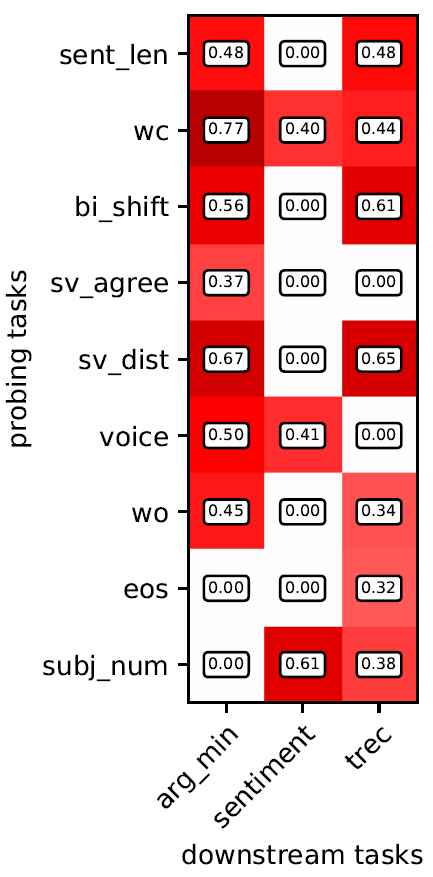
\includegraphics[scale=0.25]{images/spearman_corr_en_f1}
		\end{center}
	\end{minipage}
	\hfill
	\begin{minipage}{0.69\textwidth}
		\begin{itemize}\setlength\itemsep{1em}
			\item[] \highlight{English language}
			\item \caps{WC} has high positive correlations \textit{(intuitive)}
			\item \caps{TREC} is correlated positively with \textbf{almost all probing tasks} \textit{(found by Conneau.2018)}, also \caps{ArgMin}
			\item \caps{Senti} is less connected to probing tasks
			\item No negative correlations
		\end{itemize}
		\vfill
		{\footnotesize \textcolor{red}{positive} / \textcolor{blue}{negative} correlations}
	\end{minipage}
\end{frame}

% Correlations of Probing and Downstream Tasks
\begin{frame}{Correlations of Probing and Downstream Tasks}{}
	\vspace*{-4mm}
	\begin{minipage}{0.29\textwidth}
		\begin{center}
			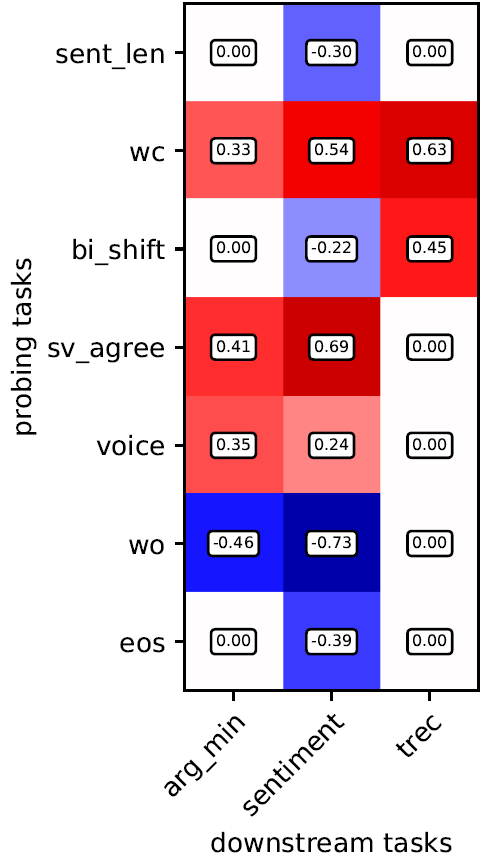
\includegraphics[scale=0.25]{images/spearman_corr_ka_f1}
		\end{center}
	\end{minipage}
	\hfill
	\begin{minipage}{0.69\textwidth}
		\begin{itemize}\setlength\itemsep{1em}
			\item[] \highlight{Georgian language}
			\item \caps{WC} has high positive correlations
			\item Many correlations \textbf{below an absolute value of 0.20 or negative}
			\item \caps{WO} is negatively correlated \\ \textit{(flexible word order in KA)}
			\item \highlight{Correlations are language-dependent!}
		\end{itemize}
		\vfill
		{\footnotesize \textcolor{red}{positive} / \textcolor{blue}{negative} correlations}
	\end{minipage}
\end{frame}


% Stability Analysis
% ===============================================
\section{Stability Analysis}
\divider{Stability Analysis}

% Stability Analysis
\begin{frame}{Stability Analysis}{}
	\vspace*{-4mm}
	\begin{itemize}\setlength\itemsep{1em}
		\item Discrepancies with the literature were found
		\item Different evaluation setups: \\ \vspace*{2mm}
		\begin{tabbing}
			\hspace*{3cm}\=\hspace*{2.5cm}\=\hspace*{2cm}\=\kill
			\texttt{Size}			\>	10k	  		\>	$\Leftrightarrow$ 	\>	90k+					\\[2mm]
			\texttt{Class balance}		\>	imbalanced	\>	$\Leftrightarrow$ 	\>	(im)balanced			\\[2mm]
			\texttt{Classifier}		\>	MLP 			\>	$\Leftrightarrow$ 	\>	MLP / Logistic regression	\\[2mm]
			\texttt{HP tuning}		\>	no 			\>	$\Leftrightarrow$ 	\>	yes (sometimes no)
		\end{tabbing}
		\item \highlight{A stability analysis is performed in order to investigate the effects of these factors}
		\item The word content task (English) is used as an example
	\end{itemize}
\end{frame}

% Stability across Classifiers
\begin{frame}{Stability across Classifiers}{}
	\vspace*{-4mm}
	\centering
	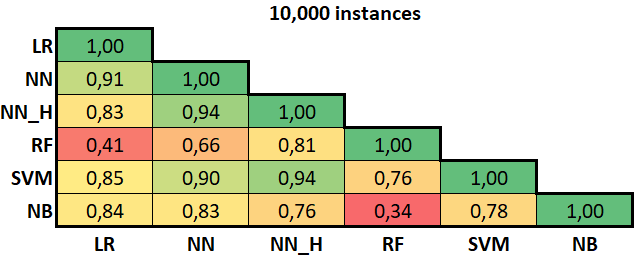
\includegraphics[scale=0.4]{images/corr_wc_en_10000}

	\vspace*{5mm}

	\begin{itemize}\setlength\itemsep{1em}
		\item Rankings are quite unstable, especially for \texttt{RF} classifier
		\item \texttt{NN} and \texttt{LR} are similar, also \texttt{NN} and \texttt{NN\_H}
		\item \highlight{Recommendation: Use a neural architecture} (outperforms other classifiers)
	\end{itemize}
\end{frame}

% Stability across Data Set Sizes
\begin{frame}{Stability across Data Set Sizes}{}
	\begin{minipage}{0.32\textwidth}
		\centering
		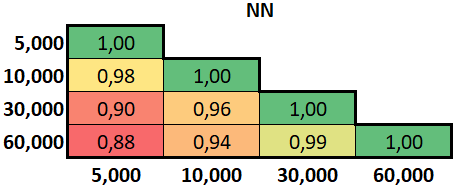
\includegraphics[scale=0.3]{images/corr_wc_en_nn}
	\end{minipage}
	\hfill
	\begin{minipage}{0.32\textwidth}
		\centering
		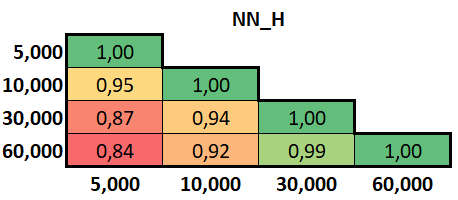
\includegraphics[scale=0.3]{images/corr_wc_en_nn_h}
	\end{minipage}
	\hfill
	\begin{minipage}{0.32\textwidth}
		\centering
		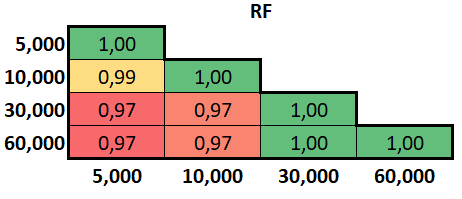
\includegraphics[scale=0.3]{images/corr_wc_en_rf}
	\end{minipage}

	\vspace*{5mm}

	\begin{itemize}\setlength\itemsep{1em}
		\item Correlations between 5k $\Leftrightarrow$ \{ 10k, 30k, 60k \} decrease
		\item However, high correlations for \texttt{RF} (less data sufficient for stable ranking)
		\item Correlations between 30k $\Leftrightarrow$ 60k close to 1.0
		\item \highlight{Recommendation: Use at least 30k instances}
	\end{itemize}
\end{frame}

% Effects of Class Balance and HP Tuning
\begin{frame}{Effects of Class Balance and HP Tuning}{}
	\vspace*{-8mm}
	\begin{figure}[h]
%\begin{minipage}{0.49\textwidth}
\begin{tikzpicture}[scale=0.95,every node/.style={scale=0.85}]
	\begin{axis}[
    		title=\textbf{Class (im-)balance (10k)},
		ylabel=$\Delta$ F1 score,
		scale only axis,
		clip=false,
		separate axis lines,
		xtick={1,2,3,4,5,6,7,8,9,10,11,12},
        	x tick style={draw=none},
        	xticklabels={Average,p-Means,SIF,GEM,Hier. pooling,BOREP,rand. BiLSTM,InferSent,Quick-Th.,sent2vec,BERT,LASER},
		xticklabels={,,},
		width=8.5cm,height=1.5cm,
		tick label style={font=\footnotesize},
		xticklabel style={rotate=90},
		ymajorgrids,
    		grid style={line width=.1pt, draw=gray!10},
		ymin=0,
		every axis plot/.append style={
          		ybar,
          		bar width=8.0,
          		bar shift=0.5pt,
			fill
		},
		scaled y ticks=false,
		y tick label style={
        		/pgf/number format/.cd,
            		fixed,
            		fixed zerofill,
            		precision=2,
        		/tikz/.cd
    		}
	]

		\addplot[draw=black,fill=blue] coordinates {(1,0.21)};
     	 	\addplot[draw=black,fill=blue!80] coordinates {(2,0.20)};
      		\addplot[draw=black,fill=blue!60] coordinates {(3,0.24)};
      		\addplot[draw=black,fill=blue!40] coordinates {(4,0.17)};
		\addplot[draw=black,fill=blue!20] coordinates {(5,0.29)};
     	 	\addplot[draw=black,fill=gray] coordinates {(6,0.25)};
      		\addplot[draw=black,fill=lightgray] coordinates {(7,0.23)};
      		\addplot[draw=black,fill=red] coordinates {(8,0.07)};
     	 	\addplot[draw=black,fill=red!80] coordinates {(9,0.06)};
      		\addplot[draw=black,fill=red!60] coordinates {(10,0.22)};
      		\addplot[draw=black,fill=red!40] coordinates {(11,0.05)};
		\addplot[draw=black,fill=red!20] coordinates {(12,0.09)};
	\end{axis}
\end{tikzpicture}
%\end{minipage}

%\begin{minipage}{0.49\textwidth}
\begin{tikzpicture}[scale=0.95,every node/.style={scale=0.85}]
	\begin{axis}[
    		title=\textbf{(No) hyper-parameter tuning (10k)},
		ylabel=$\Delta$ F1 score,
		scale only axis,
		clip=false,
		separate axis lines,
		xtick={1,2,3,4,5,6,7,8,9,10,11,12},
        	x tick style={draw=none},
        	xticklabels={Average,p-Means,SIF,GEM,Hier. pooling,BOREP,rand. BiLSTM,InferSent,Quick-Th.,sent2vec,BERT,LASER},
		width=8.5cm,height=1.5cm,
		tick label style={font=\footnotesize},
		xticklabel style={rotate=90},
		ymajorgrids,
    		grid style={line width=.1pt, draw=gray!10},
		ymin=0,
		every axis plot/.append style={
          		ybar,
          		bar width=8.0,
          		bar shift=0.5pt,
			fill
		},
		scaled y ticks=false,
		y tick label style={
        		/pgf/number format/.cd,
            		fixed,
            		fixed zerofill,
            		precision=2,
        		/tikz/.cd
    		}
	]

		\addplot[draw=black,fill=blue] coordinates {(1,0.05)};
     	 	\addplot[draw=black,fill=blue!80] coordinates {(2,0.02)};
      		\addplot[draw=black,fill=blue!60] coordinates {(3,0.05)};
      		\addplot[draw=black,fill=blue!40] coordinates {(4,0.03)};
		\addplot[draw=black,fill=blue!20] coordinates {(5,0.03)};
     	 	\addplot[draw=black,fill=gray] coordinates {(6,0.01)};
      		\addplot[draw=black,fill=lightgray] coordinates {(7,0.05)};
      		\addplot[draw=black,fill=red] coordinates {(8,0.01)};
     	 	\addplot[draw=black,fill=red!80] coordinates {(9,0.00)};
      		\addplot[draw=black,fill=red!60] coordinates {(10,0.01)};
      		\addplot[draw=black,fill=red!40] coordinates {(11,0.01)};
		\addplot[draw=black,fill=red!20] coordinates {(12,0.02)};
	\end{axis}
\end{tikzpicture}
%\end{minipage}
%
%\vspace*{4mm}
%\begin{minipage}{0.49\textwidth}
%\begin{tikzpicture}[scale=0.75,every node/.style={scale=0.85}]
%	\begin{axis}[
%    		title=\textbf{NN $\leftrightarrow$ NN\_H (10k)},
%		ylabel=$\Delta$ F1 score,
%		scale only axis,
%		clip=false,
%		separate axis lines,
%		xtick={1,2,3,4,5,6,7,8,9,10,11,12},
%        	x tick style={draw=none},
%        	xticklabels={Average,p-Means,SIF,GEM,Hier. pooling,BOREP,rand. BiLSTM,InferSent,Quick-Th.,sent2vec,BERT,LASER},
%		width=6.5cm,height=2cm,
%		tick label style={font=\footnotesize},
%		xticklabel style={rotate=90},
%		ymajorgrids,
%    		grid style={line width=.1pt, draw=gray!10},
%		every axis plot/.append style={
%          		ybar,
%          		bar width=8.0,
%          		bar shift=0.5pt,
%			fill
%		},
%		scaled y ticks=false,
%		y tick label style={
%        		/pgf/number format/.cd,
%            		fixed,
%            		fixed zerofill,
%            		precision=2,
%        		/tikz/.cd
%    		}
%	]
%
%		\addplot[draw=black,fill=blue] coordinates {(1,-0.04)};
%     	 	\addplot[draw=black,fill=blue!80] coordinates {(2,-0.03)};
%      		\addplot[draw=black,fill=blue!60] coordinates {(3,-0.01)};
%      		\addplot[draw=black,fill=blue!40] coordinates {(4,0.01)};
%		\addplot[draw=black,fill=blue!20] coordinates {(5,-0.04)};
%     	 	\addplot[draw=black,fill=gray] coordinates {(6,-0.01)};
%      		\addplot[draw=black,fill=lightgray] coordinates {(7,-0.08)};
%      		\addplot[draw=black,fill=red] coordinates {(8,-0.02)};
%     	 	\addplot[draw=black,fill=red!80] coordinates {(9,-0.02)};
%      		\addplot[draw=black,fill=red!60] coordinates {(10,0.00)};
%      		\addplot[draw=black,fill=red!40] coordinates {(11,0.02)};
%		\addplot[draw=black,fill=red!20] coordinates {(12,-0.08)};
%	\end{axis}
%\end{tikzpicture}
%\end{minipage}
%\hfill
%\begin{minipage}{0.49\textwidth}
%\begin{tikzpicture}[scale=0.75,every node/.style={scale=0.85}]
%	\begin{axis}[
%    		title=\textbf{Size (10k $\leftrightarrow$ 30k)},
%		scale only axis,
%		clip=false,
%		separate axis lines,
%		xtick={1,2,3,4,5,6,7,8,9,10,11,12},
%        	x tick style={draw=none},
%        	xticklabels={Average,p-Means,SIF,GEM,Hier. pooling,BOREP,rand. BiLSTM,InferSent,Quick-Th.,sent2vec,BERT,LASER},
%		width=6.5cm,height=2cm,
%		tick label style={font=\footnotesize},
%		xticklabel style={rotate=90},
%		ymajorgrids,
%    		grid style={line width=.1pt, draw=gray!10},
%		ymin=0,
%		every axis plot/.append style={
%          		ybar,
%          		bar width=8.0,
%          		bar shift=0.5pt,
%			fill
%		},
%		scaled y ticks=false,
%		y tick label style={
%        		/pgf/number format/.cd,
%            		fixed,
%            		fixed zerofill,
%            		precision=2,
%        		/tikz/.cd
%    		}
%	]
%
%		\addplot[draw=black,fill=blue] coordinates {(1,0.09)};
%     	 	\addplot[draw=black,fill=blue!80] coordinates {(2,0.08)};
%      		\addplot[draw=black,fill=blue!60] coordinates {(3,0.07)};
%      		\addplot[draw=black,fill=blue!40] coordinates {(4,0.01)};
%		\addplot[draw=black,fill=blue!20] coordinates {(5,0.08)};
%     	 	\addplot[draw=black,fill=gray] coordinates {(6,0.08)};
%      		\addplot[draw=black,fill=lightgray] coordinates {(7,0.13)};
%      		\addplot[draw=black,fill=red] coordinates {(8,0.02)};
%     	 	\addplot[draw=black,fill=red!80] coordinates {(9,0.05)};
%      		\addplot[draw=black,fill=red!60] coordinates {(10,0.01)};
%      		\addplot[draw=black,fill=red!40] coordinates {(11,0.04)};
%		\addplot[draw=black,fill=red!20] coordinates {(12,0.03)};
%	\end{axis}
%\end{tikzpicture}
%\end{minipage}
\end{figure}
\end{frame}

% Summary
% ===============================================
\section{Summary}
\divider{Summary}

% Summary
\begin{frame}{Summary}{}
	\vspace*{-4mm}
	\begin{itemize}\setlength\itemsep{1em}
		\item The gap between trained encoders and compositional models \textbf{vanishes in low-resource languages}
		\item Correlations in English and Georgian differ (e.\,g. no word order in Georgian)
		\item Nevertheless, the \textbf{results should be treated with caution}:
		\begin{itemize}\setlength\itemsep{1em}
			\item Use balanced data sets \textit{(considerable impact on ranking)}
			\item Use at least 30k instances
			\item Use an MLP with hyper-parameter tuning
		\end{itemize}
		\item \textbf{The evaluation should be agnostic to factors like class balance or data set size} \textit{(probing tasks suboptimal?)}
			\highlight{$\rightarrow$ future research}
	\end{itemize}
\end{frame}

% Thank you Page
\begin{frame}[plain]
	\vfill\centering
	\begin{tcolorbox}[width=4in,interior hidden,boxsep=5pt,left=0pt,right=0pt,top=2mm,
		bottom=2mm,sharp corners,colback=tud1a!40,colframe=tud1a]%%
		\centering
		\Large\textbf{Thank you very much for your attention!}
	\end{tcolorbox}
	\vfill
	\begin{center}\parbox{0cm}{
	{\footnotesize
	\begin{tabbing}
		\hspace*{3.5cm}\=\kill
		\textbf{Presenter:} 	\>	Daniel Wehner 						\\[2mm]
		\textbf{Date:}		\>	October 15, 2019 					\\[2mm]
		\textbf{Topic:}		\>	Interpretability of sentence embeddings 	\\
						\>	in low-resource languages 				\\
	\end{tabbing}}}
	\end{center}
	\vfill
	\centering
	
\includegraphics[scale=0.8]{tud_logo}
	\vfill
\end{frame}

% Universal Dependencies - Example
\begin{frame}{Universal Dependencies - Example}{}
	% UD example
	\begin{figure}[h]
\footnotesize
\begin{tabbing}
\hspace*{0.5cm}\=\hspace*{1.75cm}\=\hspace*{1.75cm}\=\hspace*{1cm}\=\hspace*{5.25cm}\=\kill
1	\>	But			\>	but					\>	\texttt{CC}		\>	\_											\>	\texttt{8:cc}					\\[1.5mm]
2	\>	in 			\>	in					\>	\texttt{IN} 		\>	\_											\>	\texttt{4:case}					\\[1.5mm]
3	\>	my			\>	my					\>	\texttt{PRP\$}	\>	\texttt{Number=Sing|Person=1|Poss=Yes}				\>	\texttt{4:nmod:poss}				\\[1.5mm]
4	\>	view			\>	view 					\>	\texttt{NN}		\>	\texttt{Number=Sing}								\>	\texttt{8:obl}					\\[1.5mm]
5	\>	it 			\>	it					\>	\texttt{PRP}	\> 	\texttt{Case=Nom|Gender=Neut|Number=Sing}			\>	\texttt{8:nsubj}					\\[1.5mm]
6	\>	is			\>	be					\>	\texttt{VBZ}	\>	\texttt{Mood=Ind|Number=Sing|Person=3}				\>	\texttt{8:cop}					\\[1.5mm]
7	\>	highly		\>	highly				\>	\texttt{RB}		\>	\_											\>	\texttt{8:advmod}				\\[1.5mm]
8	\>	significant 		\>	significant				\>	\texttt{JJ}		\>	\texttt{Degree=Pos}								\>	\texttt{0:root}					\\[1.5mm]
9	\>	.			\>	.					\>	\texttt{.}		\>	\_											\>	\texttt{8:punct}
\end{tabbing}
\end{figure}
\end{frame}

% Winner Statistics
\begin{frame}{Winner Statistics (Probing Tasks)}{}
	\vspace*{-7mm}
	\begin{figure}[h]
\begin{minipage}{0.30\textwidth}
\begin{tikzpicture}[scale=0.75,every node/.style={scale=0.85}]
	\begin{axis}[
    		title=\textbf{Top-three scores (EN)},
		scale only axis,
		clip=false,
		separate axis lines,
		xtick={1,2,3,4,5,6,7,8,9,10,11,12},
        	x tick style={draw=none},
        	xticklabels={Avg,p-Means,SIF,GEM,H. pooling,BOREP,r. BiLSTM,InferSent,Quick-Th.,sent2vec,BERT,LASER},
		width=4cm,height=2cm,
		tick label style={font=\footnotesize},
		xticklabel style={rotate=90},
		ymajorgrids,
    		grid style={line width=.1pt, draw=gray!10},
		ymin=0,ymax=1,
		every axis plot/.append style={
          		ybar,
          		bar width=6.0,
          		bar shift=0.5pt,
			fill
		},
		scaled y ticks=false,
		y tick label style={
        		/pgf/number format/.cd,
            		fixed,
            		fixed zerofill,
            		precision=2,
        		/tikz/.cd
    		}
	]

		\addplot[draw=black,fill=blue] coordinates {(1,0.00)};
     	 	\addplot[draw=black,fill=blue!80] coordinates {(2,0.33)};
      		\addplot[draw=black,fill=blue!60] coordinates {(3,0.00)};
      		\addplot[draw=black,fill=blue!40] coordinates {(4,0.00)};
		\addplot[draw=black,fill=blue!20] coordinates {(5,0.00)};
     	 	\addplot[draw=black,fill=gray] coordinates {(6,0.00)};
      		\addplot[draw=black,fill=lightgray] coordinates {(7,0.33)};
      		\addplot[draw=black,fill=red] coordinates {(8,0.78)};
     	 	\addplot[draw=black,fill=red!80] coordinates {(9,0.56)};
      		\addplot[draw=black,fill=red!60] coordinates {(10,0.00)};
      		\addplot[draw=black,fill=red!40] coordinates {(11,0.22)};
		\addplot[draw=black,fill=red!20] coordinates {(12,0.78)};
	\end{axis}
\end{tikzpicture}
\end{minipage}
\hfill
\begin{minipage}{0.30\textwidth}
\begin{tikzpicture}[scale=0.75,every node/.style={scale=0.85}]
	\begin{axis}[
    		title=\textbf{Top-three scores (DE)},
		scale only axis,
		clip=false,
		separate axis lines,
		xtick={1,2,3,4,5,6,7,8,9,10,11,12},
        	x tick style={draw=none},
        	xticklabels={Avg,p-Means,SIF,GEM,H. pooling,BOREP,r. BiLSTM,InferSent,Quick-Th.,sent2vec,BERT,LASER},
		width=4cm,height=2cm,
		tick label style={font=\footnotesize},
		xticklabel style={rotate=90},
		ymajorgrids,
    		grid style={line width=.1pt, draw=gray!10},
		ymin=0,ymax=1,
		every axis plot/.append style={
          		ybar,
          		bar width=6.0,
          		bar shift=0.5pt,
			fill
		},
		scaled y ticks=false,
		y tick label style={
        		/pgf/number format/.cd,
            		fixed,
            		fixed zerofill,
            		precision=2,
        		/tikz/.cd
    		}
	]

		\addplot[draw=black,fill=blue] coordinates {(1,0.11)};
     	 	\addplot[draw=black,fill=blue!80] coordinates {(2,0.11)};
      		\addplot[draw=black,fill=blue!60] coordinates {(3,0.00)};
      		\addplot[draw=black,fill=blue!40] coordinates {(4,0.11)};
		\addplot[draw=black,fill=blue!20] coordinates {(5,0.00)};
     	 	\addplot[draw=black,fill=gray] coordinates {(6,0.11)};
      		\addplot[draw=black,fill=lightgray] coordinates {(7,0.22)};
      		\addplot[draw=black,fill=red] coordinates {(8,0.22)};
     	 	\addplot[draw=black,fill=red!80] coordinates {(9,0.56)};
      		\addplot[draw=black,fill=red!60] coordinates {(10,0.44)};
      		\addplot[draw=black,fill=red!40] coordinates {(11,0.33)};
		\addplot[draw=black,fill=red!20] coordinates {(12,0.78)};
	\end{axis}
\end{tikzpicture}
\end{minipage}
\hfill
\begin{minipage}{0.30\textwidth}
\begin{tikzpicture}[scale=0.75,every node/.style={scale=0.85}]
	\begin{axis}[
    		title=\textbf{Top-three scores (RU)},
		scale only axis,
		clip=false,
		separate axis lines,
		xtick={1,2,3,4,5,6,7,8,9,10,11,12},
        	x tick style={draw=none},
        	xticklabels={Avg,p-Means,SIF,GEM,H. pooling,BOREP,r. BiLSTM,InferSent,Quick-Th.,sent2vec,BERT,LASER},
		width=4cm,height=2cm,
		tick label style={font=\footnotesize},
		xticklabel style={rotate=90},
		ymajorgrids,
    		grid style={line width=.1pt, draw=gray!10},
		ymin=0,ymax=1,
		every axis plot/.append style={
          		ybar,
          		bar width=6.0,
          		bar shift=0.5pt,
			fill
		},
		scaled y ticks=false,
		y tick label style={
        		/pgf/number format/.cd,
            		fixed,
            		fixed zerofill,
            		precision=2,
        		/tikz/.cd
    		}
	]

		\addplot[draw=black,fill=blue] coordinates {(1,0.33)};
     	 	\addplot[draw=black,fill=blue!80] coordinates {(2,0.33)};
      		\addplot[draw=black,fill=blue!60] coordinates {(3,0.11)};
      		\addplot[draw=black,fill=blue!40] coordinates {(4,0.11)};
		\addplot[draw=black,fill=blue!20] coordinates {(5,0.00)};
     	 	\addplot[draw=black,fill=gray] coordinates {(6,0.00)};
      		\addplot[draw=black,fill=lightgray] coordinates {(7,0.33)};
      		\addplot[draw=black,fill=red] coordinates {(8,0.11)};
     	 	\addplot[draw=black,fill=red!80] coordinates {(9,0.56)};
      		\addplot[draw=black,fill=red!60] coordinates {(10,0.22)};
      		\addplot[draw=black,fill=red!40] coordinates {(11,0.33)};
		\addplot[draw=black,fill=red!20] coordinates {(12,0.56)};
	\end{axis}
\end{tikzpicture}
\end{minipage}

\begin{minipage}[c]{0.30\textwidth}
\begin{tikzpicture}[scale=0.75,every node/.style={scale=0.85}]
	\begin{axis}[
    		title=\textbf{Top-three scores (TR)},
		scale only axis,
		clip=false,
		separate axis lines,
		xtick={1,2,3,4,5,6,7,8,9,10,11,12},
        	x tick style={draw=none},
        	xticklabels={Avg,p-Means,SIF,GEM,H. pooling,BOREP,r. BiLSTM,InferSent,Quick-Th.,sent2vec,BERT,LASER},
		width=4cm,height=2cm,
		tick label style={font=\footnotesize},
		xticklabel style={rotate=90},
		ymajorgrids,
    		grid style={line width=.1pt, draw=gray!10},
		ymin=0,ymax=1,
		every axis plot/.append style={
          		ybar,
          		bar width=6.0,
          		bar shift=0.5pt,
			fill
		},
		scaled y ticks=false,
		y tick label style={
        		/pgf/number format/.cd,
            		fixed,
            		fixed zerofill,
            		precision=2,
        		/tikz/.cd
    		}
	]

		\addplot[draw=black,fill=blue] coordinates {(1,0.11)};
     	 	\addplot[draw=black,fill=blue!80] coordinates {(2,0.33)};
      		\addplot[draw=black,fill=blue!60] coordinates {(3,0.11)};
      		\addplot[draw=black,fill=blue!40] coordinates {(4,0.22)};
		\addplot[draw=black,fill=blue!20] coordinates {(5,0.00)};
     	 	\addplot[draw=black,fill=gray] coordinates {(6,0.00)};
      		\addplot[draw=black,fill=lightgray] coordinates {(7,0.22)};
      		\addplot[draw=black,fill=red] coordinates {(8,0.11)};
     	 	\addplot[draw=black,fill=red!80] coordinates {(9,0.44)};
      		\addplot[draw=black,fill=red!60] coordinates {(10,0.11)};
      		\addplot[draw=black,fill=red!40] coordinates {(11,0.56)};
		\addplot[draw=black,fill=red!20] coordinates {(12,0.89)};
	\end{axis}
\end{tikzpicture}
\end{minipage}
\hfill
\begin{minipage}[c]{0.30\textwidth}
\end{minipage}
\hfill
\begin{minipage}[c]{0.30\textwidth}
\begin{tikzpicture}[scale=0.75,every node/.style={scale=0.85}]
	\begin{axis}[
    		title=\textbf{Top-three scores (KA)},
		scale only axis,
		clip=false,
		separate axis lines,
		xtick={1,2,3,4,5,6,7,8,9,10,11,12},
        	x tick style={draw=none},
        	xticklabels={Avg,p-Means,SIF,GEM,H. pooling,BOREP,r. BiLSTM,InferSent,Quick-Th.,sent2vec,BERT,LASER},
		width=4cm,height=2cm,
		tick label style={font=\footnotesize},
		xticklabel style={rotate=90},
		ymajorgrids,
    		grid style={line width=.1pt, draw=gray!10},
		ymin=0,ymax=1,
		every axis plot/.append style={
          		ybar,
          		bar width=6.0,
          		bar shift=0.5pt,
			fill
		},
		scaled y ticks=false,
		y tick label style={
        		/pgf/number format/.cd,
            		fixed,
            		fixed zerofill,
            		precision=2,
        		/tikz/.cd
    		}
	]

		\addplot[draw=black,fill=blue] coordinates {(1,0.00)};
     	 	\addplot[draw=black,fill=blue!80] coordinates {(2,0.57)};
      		\addplot[draw=black,fill=blue!60] coordinates {(3,0.00)};
      		\addplot[draw=black,fill=blue!40] coordinates {(4,0.00)};
		\addplot[draw=black,fill=blue!20] coordinates {(5,0.00)};
     	 	\addplot[draw=black,fill=gray] coordinates {(6,0.14)};
      		\addplot[draw=black,fill=lightgray] coordinates {(7,0.29)};
      		\addplot[draw=black,fill=red] coordinates {(8,0.43)};
     	 	\addplot[draw=black,fill=red!80] coordinates {(9,0.29)};
      		\addplot[draw=black,fill=red!60] coordinates {(10,0.29)};
      		\addplot[draw=black,fill=red!40] coordinates {(11,0.43)};
		\addplot[draw=black,fill=red!20] coordinates {(12,0.57)};
	\end{axis}
\end{tikzpicture}
\end{minipage}
\end{figure}
\end{frame}

% Winner Statistics
\begin{frame}{Winner Statistics (Probing Tasks)}{}
	\vspace*{-7mm}
	\begin{figure}[h]
\begin{minipage}{0.30\textwidth}
\begin{tikzpicture}[scale=0.75,every node/.style={scale=0.85}]
	\begin{axis}[
    		title=\textbf{Top-three scores (EN)},
		scale only axis,
		clip=false,
		separate axis lines,
		xtick={1,2,3,4,5,6,7,8,9,10,11,12},
        	x tick style={draw=none},
        	xticklabels={Avg,p-Means,SIF,GEM,H. pooling,BOREP,r. BiLSTM,InferSent,Quick-Th.,sent2vec,BERT,LASER},
		width=4cm,height=2cm,
		tick label style={font=\footnotesize},
		xticklabel style={rotate=90},
		ymajorgrids,
    		grid style={line width=.1pt, draw=gray!10},
		ymin=0,ymax=1,
		every axis plot/.append style={
          		ybar,
          		bar width=6.0,
          		bar shift=0.5pt,
			fill
		},
		scaled y ticks=false,
		y tick label style={
        		/pgf/number format/.cd,
            		fixed,
            		fixed zerofill,
            		precision=2,
        		/tikz/.cd
    		}
	]

		\addplot[draw=black,fill=blue] coordinates {(1,0.00)};
     	 	\addplot[draw=black,fill=blue!80] coordinates {(2,0.33)};
      		\addplot[draw=black,fill=blue!60] coordinates {(3,0.00)};
      		\addplot[draw=black,fill=blue!40] coordinates {(4,0.00)};
		\addplot[draw=black,fill=blue!20] coordinates {(5,0.00)};
     	 	\addplot[draw=black,fill=gray] coordinates {(6,0.00)};
      		\addplot[draw=black,fill=lightgray] coordinates {(7,0.33)};
      		\addplot[draw=black,fill=red] coordinates {(8,0.78)};
     	 	\addplot[draw=black,fill=red!80] coordinates {(9,0.56)};
      		\addplot[draw=black,fill=red!60] coordinates {(10,0.00)};
      		\addplot[draw=black,fill=red!40] coordinates {(11,0.22)};
		\addplot[draw=black,fill=red!20] coordinates {(12,0.78)};
	\end{axis}
\end{tikzpicture}
\end{minipage}
\hfill
\begin{minipage}{0.30\textwidth}
\begin{tikzpicture}[scale=0.75,every node/.style={scale=0.85}]
	\begin{axis}[
    		title=\textbf{Top-three scores (DE)},
		scale only axis,
		clip=false,
		separate axis lines,
		xtick={1,2,3,4,5,6,7,8,9,10,11,12},
        	x tick style={draw=none},
        	xticklabels={Avg,p-Means,SIF,GEM,H. pooling,BOREP,r. BiLSTM,InferSent,Quick-Th.,sent2vec,BERT,LASER},
		width=4cm,height=2cm,
		tick label style={font=\footnotesize},
		xticklabel style={rotate=90},
		ymajorgrids,
    		grid style={line width=.1pt, draw=gray!10},
		ymin=0,ymax=1,
		every axis plot/.append style={
          		ybar,
          		bar width=6.0,
          		bar shift=0.5pt,
			fill
		},
		scaled y ticks=false,
		y tick label style={
        		/pgf/number format/.cd,
            		fixed,
            		fixed zerofill,
            		precision=2,
        		/tikz/.cd
    		}
	]

		\addplot[draw=black,fill=blue] coordinates {(1,0.11)};
     	 	\addplot[draw=black,fill=blue!80] coordinates {(2,0.11)};
      		\addplot[draw=black,fill=blue!60] coordinates {(3,0.00)};
      		\addplot[draw=black,fill=blue!40] coordinates {(4,0.11)};
		\addplot[draw=black,fill=blue!20] coordinates {(5,0.00)};
     	 	\addplot[draw=black,fill=gray] coordinates {(6,0.11)};
      		\addplot[draw=black,fill=lightgray] coordinates {(7,0.22)};
      		\addplot[draw=black,fill=red] coordinates {(8,0.22)};
     	 	\addplot[draw=black,fill=red!80] coordinates {(9,0.56)};
      		\addplot[draw=black,fill=red!60] coordinates {(10,0.44)};
      		\addplot[draw=black,fill=red!40] coordinates {(11,0.33)};
		\addplot[draw=black,fill=red!20] coordinates {(12,0.78)};
	\end{axis}
\end{tikzpicture}
\end{minipage}
\hfill
\begin{minipage}{0.30\textwidth}
\begin{tikzpicture}[scale=0.75,every node/.style={scale=0.85}]
	\begin{axis}[
    		title=\textbf{Top-three scores (RU)},
		scale only axis,
		clip=false,
		separate axis lines,
		xtick={1,2,3,4,5,6,7,8,9,10,11,12},
        	x tick style={draw=none},
        	xticklabels={Avg,p-Means,SIF,GEM,H. pooling,BOREP,r. BiLSTM,InferSent,Quick-Th.,sent2vec,BERT,LASER},
		width=4cm,height=2cm,
		tick label style={font=\footnotesize},
		xticklabel style={rotate=90},
		ymajorgrids,
    		grid style={line width=.1pt, draw=gray!10},
		ymin=0,ymax=1,
		every axis plot/.append style={
          		ybar,
          		bar width=6.0,
          		bar shift=0.5pt,
			fill
		},
		scaled y ticks=false,
		y tick label style={
        		/pgf/number format/.cd,
            		fixed,
            		fixed zerofill,
            		precision=2,
        		/tikz/.cd
    		}
	]

		\addplot[draw=black,fill=blue] coordinates {(1,0.33)};
     	 	\addplot[draw=black,fill=blue!80] coordinates {(2,0.33)};
      		\addplot[draw=black,fill=blue!60] coordinates {(3,0.11)};
      		\addplot[draw=black,fill=blue!40] coordinates {(4,0.11)};
		\addplot[draw=black,fill=blue!20] coordinates {(5,0.00)};
     	 	\addplot[draw=black,fill=gray] coordinates {(6,0.00)};
      		\addplot[draw=black,fill=lightgray] coordinates {(7,0.33)};
      		\addplot[draw=black,fill=red] coordinates {(8,0.11)};
     	 	\addplot[draw=black,fill=red!80] coordinates {(9,0.56)};
      		\addplot[draw=black,fill=red!60] coordinates {(10,0.22)};
      		\addplot[draw=black,fill=red!40] coordinates {(11,0.33)};
		\addplot[draw=black,fill=red!20] coordinates {(12,0.56)};
	\end{axis}
\end{tikzpicture}
\end{minipage}

\begin{minipage}[c]{0.30\textwidth}
\begin{tikzpicture}[scale=0.75,every node/.style={scale=0.85}]
	\begin{axis}[
    		title=\textbf{Top-three scores (TR)},
		scale only axis,
		clip=false,
		separate axis lines,
		xtick={1,2,3,4,5,6,7,8,9,10,11,12},
        	x tick style={draw=none},
        	xticklabels={Avg,p-Means,SIF,GEM,H. pooling,BOREP,r. BiLSTM,InferSent,Quick-Th.,sent2vec,BERT,LASER},
		width=4cm,height=2cm,
		tick label style={font=\footnotesize},
		xticklabel style={rotate=90},
		ymajorgrids,
    		grid style={line width=.1pt, draw=gray!10},
		ymin=0,ymax=1,
		every axis plot/.append style={
          		ybar,
          		bar width=6.0,
          		bar shift=0.5pt,
			fill
		},
		scaled y ticks=false,
		y tick label style={
        		/pgf/number format/.cd,
            		fixed,
            		fixed zerofill,
            		precision=2,
        		/tikz/.cd
    		}
	]

		\addplot[draw=black,fill=blue] coordinates {(1,0.11)};
     	 	\addplot[draw=black,fill=blue!80] coordinates {(2,0.33)};
      		\addplot[draw=black,fill=blue!60] coordinates {(3,0.11)};
      		\addplot[draw=black,fill=blue!40] coordinates {(4,0.22)};
		\addplot[draw=black,fill=blue!20] coordinates {(5,0.00)};
     	 	\addplot[draw=black,fill=gray] coordinates {(6,0.00)};
      		\addplot[draw=black,fill=lightgray] coordinates {(7,0.22)};
      		\addplot[draw=black,fill=red] coordinates {(8,0.11)};
     	 	\addplot[draw=black,fill=red!80] coordinates {(9,0.44)};
      		\addplot[draw=black,fill=red!60] coordinates {(10,0.11)};
      		\addplot[draw=black,fill=red!40] coordinates {(11,0.56)};
		\addplot[draw=black,fill=red!20] coordinates {(12,0.89)};
	\end{axis}
\end{tikzpicture}
\end{minipage}
\hfill
\begin{minipage}[c]{0.30\textwidth}
\end{minipage}
\hfill
\begin{minipage}[c]{0.30\textwidth}
\begin{tikzpicture}[scale=0.75,every node/.style={scale=0.85}]
	\begin{axis}[
    		title=\textbf{Top-three scores (KA)},
		scale only axis,
		clip=false,
		separate axis lines,
		xtick={1,2,3,4,5,6,7,8,9,10,11,12},
        	x tick style={draw=none},
        	xticklabels={Avg,p-Means,SIF,GEM,H. pooling,BOREP,r. BiLSTM,InferSent,Quick-Th.,sent2vec,BERT,LASER},
		width=4cm,height=2cm,
		tick label style={font=\footnotesize},
		xticklabel style={rotate=90},
		ymajorgrids,
    		grid style={line width=.1pt, draw=gray!10},
		ymin=0,ymax=1,
		every axis plot/.append style={
          		ybar,
          		bar width=6.0,
          		bar shift=0.5pt,
			fill
		},
		scaled y ticks=false,
		y tick label style={
        		/pgf/number format/.cd,
            		fixed,
            		fixed zerofill,
            		precision=2,
        		/tikz/.cd
    		}
	]

		\addplot[draw=black,fill=blue] coordinates {(1,0.00)};
     	 	\addplot[draw=black,fill=blue!80] coordinates {(2,0.57)};
      		\addplot[draw=black,fill=blue!60] coordinates {(3,0.00)};
      		\addplot[draw=black,fill=blue!40] coordinates {(4,0.00)};
		\addplot[draw=black,fill=blue!20] coordinates {(5,0.00)};
     	 	\addplot[draw=black,fill=gray] coordinates {(6,0.14)};
      		\addplot[draw=black,fill=lightgray] coordinates {(7,0.29)};
      		\addplot[draw=black,fill=red] coordinates {(8,0.43)};
     	 	\addplot[draw=black,fill=red!80] coordinates {(9,0.29)};
      		\addplot[draw=black,fill=red!60] coordinates {(10,0.29)};
      		\addplot[draw=black,fill=red!40] coordinates {(11,0.43)};
		\addplot[draw=black,fill=red!20] coordinates {(12,0.57)};
	\end{axis}
\end{tikzpicture}
\end{minipage}
\end{figure}
\end{frame}

% Effect of Hyper-Parameter Tuning (other Tasks)
\begin{frame}{Effect of Hyper-Parameter Tuning (other Tasks)}{}
	\begin{table}[H]
	\centering
	\renewcommand{\arraystretch}{1.0}
	\scalebox{0.9}{
	\begin{tabular}{| l ? c | c | c |}
		\hline
		\rowcolor{tud1a}
		\multicolumn{4}{| c |}{\textcolor{white}{\textbf{Effect of hyper-parameter tuning on other tasks}}}
		\\ \hline
		\rowcolor{tud1a!50}
								&
		$\bm{\Delta}$ \caps{Senti} 	&
		$\bm{\Delta}$ \caps{Voice} 	&
		$\bm{\Delta}$ \caps{SubjNum}
		\\ \hline\hline
		Vanilla average		& 0.02 & 0.00 & 0.00 \\ \hline
		p-Means 			& 0.00 & 0.02 & 0.03 \\ \hline
		BOREP 			& 0.00 & 0.02 & 0.03 \\ \hline
		Random BiLSTM 	& 0.00 & 0.01 & 0.00 \\ \hline
		InferSent 			& 0.05 & 0.03 & 0.03 \\ \hline
		Quick-Thought 		& 0.03 & 0.02 & 0.04 \\ \hline
		sent2vec 			& 0.00 & 0.00 & 0.01 \\ \hline
		BERT 			& 0.01 & 0.02 & 0.02 \\ \hline
		LASER 			& 0.01 & 0.03 & 0.02 \\ \hline
	\end{tabular}}
\end{table}
\end{frame}

% Stability Analysis: Effects on Ranking
\begin{frame}{Stability Analysis: Effects on Ranking}{}
	\vspace*{-8mm}
	\begin{table}[h]
	\centering
	\renewcommand{\arraystretch}{1.3}
	\scalebox{0.65}{
	\begin{tabular}{l c c c c c c c c c c c c}
									&
		\rotff{\textbf{Vanilla average}}		&
		\rotff{\textbf{p-Means}}			&
		\rotff{\textbf{SIF}}				&
		\rotff{\textbf{GEM}}				&
		\rotff{\textbf{hier. pooling}}		&
		\rotff{\textbf{BOREP}}			&
		\rotff{\textbf{Random BiLSTM}}		&
		\rotff{\textbf{InferSent}}			&
		\rotff{\textbf{Quick-Thought}}		&
		\rotff{\textbf{sent2vec}}			&
		\rotff{\textbf{BERT}}				&
		\rotff{\textbf{LASER}}				\\ \hline
		\multicolumn{13}{l}{\ding{182} \textbf{class (im-)balance}}											\\
		\textbf{Ranking} \textit{(imbalanced, 10k)}				& 8 & 6 & 7 & 5 & 12 & 9 & 11 & 1 & 3 & 4 & 9 & 2 	\\
		\textbf{Ranking} \textit{(balanced, 10k)}				& 8 & 7 & 6 & 5 & 11 & 9 & 10 & 2 & 4 & 1 & 12 & 3 	\\
		& \multicolumn{12}{c}{\textbf{Spearman correlation: 0.91}}											\\ \hline
		\multicolumn{13}{l}{\ding{183} \textbf{(no) hyper-parameter tuning}}									\\
		\textbf{Ranking} \textit{(balanced, no optimization, 10k)}	& 8 & 7 & 6 & 5 & 11 & 9 & 10 & 2 & 4 & 1 & 12 & 3 	\\
		\textbf{Ranking} \textit{(balanced, optimization, 10k)}		& 7 & 8 & 4 & 4 & 11 & 10 & 9 & 2 & 6 & 1 & 12 & 3 	\\
		& \multicolumn{12}{c}{\textbf{Spearman correlation: 0.95}}											\\ \hline
		\multicolumn{13}{l}{\ding{185} \textbf{size (30k $\leftrightarrow$ 60k)}}								\\
		\textbf{Ranking} \textit{(balanced, 30k)}				& 6 & 6 & 5 & 8 & 11 & 10 & 9 & 2 & 4 & 1 & 12 & 3 	\\
		\textbf{Ranking} \textit{(balanced, 60k)}				& 7 & 5 & 5 & 9 & 11 & 10 & 8 & 1 & 4 & 1 & 12 & 3 	\\
		& \multicolumn{12}{c}{\textbf{Spearman correlation: 0.98}}											\\ \hline
	\end{tabular}}
\end{table}
\end{frame}

\end{document}
